\documentclass[11pt]{article}
\usepackage[margin=1in]{geometry}
\usepackage{amsmath}
\usepackage{booktabs}
\usepackage{graphicx}
\usepackage{float}
\usepackage[hidelinks]{hyperref}
\emergencystretch=3em
\graphicspath{{figs/}}

\newcommand{\code}[1]{\texttt{#1}}

\title{Vibration frequencies of the DTU10MW blade in the three vibration regions}
\author{Ilan Upfal}
\date{29 October 2026, revised 20 November 2026}

\begin{document}
\maketitle

\section*{Summary}

For each production run and each of the three motor-angle regions where the
blade vibrates (R1, R2, R3), we took the accelerometer spectrum at the angle
of strongest vibration and found its dominant frequency. We then compared
those frequencies across runs, both in hertz and as a Strouhal number
$St = f\bar{c}/U$, to see whether the vibration is set by the blade or by the
flow.

\begin{enumerate}
  \item \textbf{R1 (motor 105--135$^\circ$) vibrates at fixed frequencies.}
        Edgewise, 13 of the 17 vibrating runs (sensor~4) sit at
        $112 \pm 3$\,Hz while the flow speed doubles (3.4 to 6.9\,m/s).
        Flapwise, most runs sit at 130--150\,Hz. The frequency does not follow
        the flow, so this is a structural resonance excited by the flow.
  \item \textbf{R2 (155--185$^\circ$) follows the flow.} Most R2 peaks rise
        with flow speed, from 77\,Hz at 2.6\,m/s to 224\,Hz at 7.8\,m/s, at a
        nearly constant $St \approx 0.4$. This is what a flow-driven forcing
        such as vortex shedding looks like. A separate group of three fast runs
        vibrates at $\sim$290\,Hz.
  \item \textbf{R3 (195--225$^\circ$) vibrates at about 100\,Hz} in both
        directions, from 4.3 to 7.8\,m/s, and only in the fastest runs.
  \item \textbf{The root and tip sensors mostly agree.} For runs flagged by
        both sensor~1 (root) and sensor~4 (tip), the peak frequencies agree to
        within 5\,Hz in 37 of 48 cases. The main exception is R1 flapwise,
        where the root sensor often peaks at the $\sim$110\,Hz edgewise
        frequency instead. Sensor~4 flags more runs because the tip moves
        more.
\end{enumerate}

%======================================================================
\section{Methods}
%======================================================================

\subsection{Data}

The data are the 32 production runs of 6--15 October 2026
(\code{data/Production\_10-8-26}). Each run holds the blade at a fixed tunnel
pressure and fan setting and steps the motor through a sweep of angles,
recording 60\,s of acceleration at each angle from four accelerometers along
the span (S1 at the root to S4 at the tip). The tunnel is pressurized, so the
gas density ranges from 32 to 114\,kg/m$^3$ and the flow speed $U$ from 2.5 to
7.8\,m/s.

This analysis uses the 22 runs whose sweep covers at least 95\% of the full
circle (the same runs as the design-space figure,
\code{figures/design\_space}). The ten partial sweeps are left out because the
quiet baseline used to flag vibration (Section~\ref{sec:flags}) is not
reliable for them.

\paragraph{Directions.} Each accelerometer measures along three axes. From the
ring-down tests (\code{reports/ringdown}), flicking the tip flapwise rings
mostly in $z$ and flicking it edgewise mostly in $y$; $x$ is spanwise and
barely moves. We therefore call $y$ \emph{edgewise} and $z$ \emph{flapwise}.
The flicks are not pure, so each axis also picks up some motion in the other
direction.

\paragraph{Flow parameters.} Each run is characterized by
\begin{align*}
  Re &= \frac{\rho U \bar{c}}{\mu}, &
  Ca_e &= \frac{\rho U^2 b^4}{B_e}, &
  St &= \frac{f \bar{c}}{U},
\end{align*}
with measured density $\rho$, viscosity $\mu$ and speed $U$, mean chord
$\bar{c} = 13.8$\,mm, span $b = 0.28$\,m and edgewise bending stiffness $B_e$.
$Re$ ranges from $0.6$ to $3.3\times10^5$ and $Ca_e$ from 5 to 90 over the 22
runs. Because both rise with $U$ and with pressure, they are strongly
correlated in this test matrix.

\subsection{Spectra}

For every angle of every run, \code{extract\_run\_summary.py} (version 1.4)
computes the power spectral density (PSD) of each accelerometer axis with
Welch's method (segments of 2048 samples, Hann window, 0.73\,Hz resolution).
Two details of the accelerometer timing matter:

\begin{itemize}
  \item \textbf{Sample rate.} The sensors sample at 1493\,Hz, measured by the
        vendor, not at the configured 1600\,Hz. Using 1600\,Hz would put every
        frequency 7\% high.
  \item \textbf{Dropped samples.} Our read loop loses about 16 of every 100
        samples, in a gap after each read. Each sample is placed at its true
        time and the gaps are left empty, so frequencies are correct. The
        regular gaps add weak copies of each peak about 14\,Hz either side,
        carrying about 3\% of its power.
\end{itemize}
Both are described in \code{reports/accel\_sampling} and
\code{reports/pcb\_manual\_notes}. Frequencies above about 150\,Hz depend on
the exact sample rate and are uncertain by up to one copy spacing
($\sim$15\,Hz).

Each PSD is divided by $a_c^2$, where $a_c = \tfrac12 \rho U^2 \bar{c} b / m$
is the acceleration the aerodynamic load alone would give the blade mass $m$.
This makes runs at different speeds and pressures comparable. In Strouhal
form the PSD is expressed per unit $St$, so the area under each curve is still
the variance.

\subsection{Vibration regions and flags}
\label{sec:flags}

The blade vibrates strongly in three windows of motor angle, fixed for all
runs because the exact peak wanders by about $\pm10^\circ$ between tests:
R1 = 105--135$^\circ$, R2 = 155--185$^\circ$, R3 = 195--225$^\circ$. In the
blade's inflow frame (production geometry: sweep $-30^\circ$, chord
5.9$^\circ$ off perpendicular to the arm; conventions and checks in
\code{reports/angle\_check}) these are angles of attack of 113--145$^\circ$,
164$^\circ$ to $-170^\circ$ (through $\pm180^\circ$) and $-161$ to
$-133^\circ$, with inclinations of $+21$ to $+29^\circ$, $-2$ to $+12^\circ$
and $-21$ to $-7^\circ$: the flow reaches the blade roughly from the
trailing edge.

For each run, \code{angle\_metrics.py} computes a quiet baseline: the median
over the sweep of the normalized variance $\mathrm{Var}(|a|)/a_c^2$ of the
chosen sensor. A run is \emph{flagged} in a region if the largest variance
inside the window is at least ten times that baseline. Flagged runs are the
ones with real vibration in that region; unflagged runs are shown in grey and
are not used in the statistics below.

\subsection{Peak frequency}

For each run, region and direction, \code{plot\_psd.py} takes the spectrum at
the measured angle inside the window where that axis's variance is largest.
It smooths the spectrum over five bins ($\sim$3.6\,Hz) and takes the highest
point between 5 and 500\,Hz as the peak frequency $f$, and $St = f\bar{c}/U$.
The copies made by the dropped samples are always weaker than the peak they
copy, so they never win this choice.

The figures show, for one region, direction and sensor, every run's spectrum
(top) and its peak frequency against $Re$ (bottom), coloured by $Re$ or by
$Ca_e$ (\code{figures/psd\_analysis}, with sensor~4 in \code{S4/} and the
$Ca_e$-coloured versions in \code{cauchy/}). Grey curves and points are runs
not flagged in that region; for them the ``peak'' is often just the top of a
flat spectrum. All figures share the same axis limits.

\paragraph{Ring-down frequencies are not shown.} The ring-down tests found
different natural frequencies with and without a mount bolt
(\code{reports/ringdown}). That report has since concluded that the
production runs most likely had no bolt. Without it the blade has its first
flapwise mode at 55\,Hz and a first-edgewise/second-flapwise pair at 131 and
138\,Hz, and the mount has a mode at 85\,Hz. The figures carry no
natural-frequency lines.

\paragraph{How to read the results.} If a peak stays at the same frequency in
hertz as the flow speed changes, it is set by the structure: the blade
resonates at its own frequency, and its Strouhal number falls as $1/U$. If it
stays at the same Strouhal number, its frequency rises in proportion to $U$
and it is set by the flow.

%======================================================================
\section{Results}
%======================================================================

\subsection{Overview}

Table~\ref{tab:overview} lists, for each region and direction, how many of
the 22 runs are flagged and the spread of their peak frequencies.
Figure~\ref{fig:speed} plots every flagged sensor-4 peak against flow speed,
with lines of constant Strouhal number for reference.

\begin{table}[H]
  \centering
  \begin{tabular}{llcccccc}
    \toprule
    & & \multicolumn{3}{c}{Sensor 1 (root)} & \multicolumn{3}{c}{Sensor 4 (tip)} \\
    \cmidrule(lr){3-5}\cmidrule(lr){6-8}
    Region & Direction & Runs & $f$ median (Hz) & $St$ median & Runs & $f$ median (Hz) & $St$ median \\
    \midrule
    R1 & edgewise & 11 & 111 & 0.29 & 17 & 112 & 0.31 \\
       & flapwise & 11 & 135 & 0.39 & 17 & 136 & 0.39 \\
    R2 & edgewise & 10 & 189 & 0.44 & 14 & 135 & 0.41 \\
       & flapwise & 10 & 216 & 0.51 & 14 & 147 & 0.43 \\
    R3 & edgewise &  4 &  98 & 0.20 &  6 & 100 & 0.21 \\
       & flapwise &  4 &  98 & 0.20 &  6 & 100 & 0.21 \\
    \bottomrule
  \end{tabular}
  \caption{Flagged runs (of 22) and their median peak frequency and Strouhal
  number. A run is flagged in a region if its vibration there is at least ten
  times its quiet level. The R2 medians differ between sensors because R2
  mixes two groups (Section~\ref{sec:r2}) in different proportions.}
  \label{tab:overview}
\end{table}

\begin{figure}[H]
  \centering
  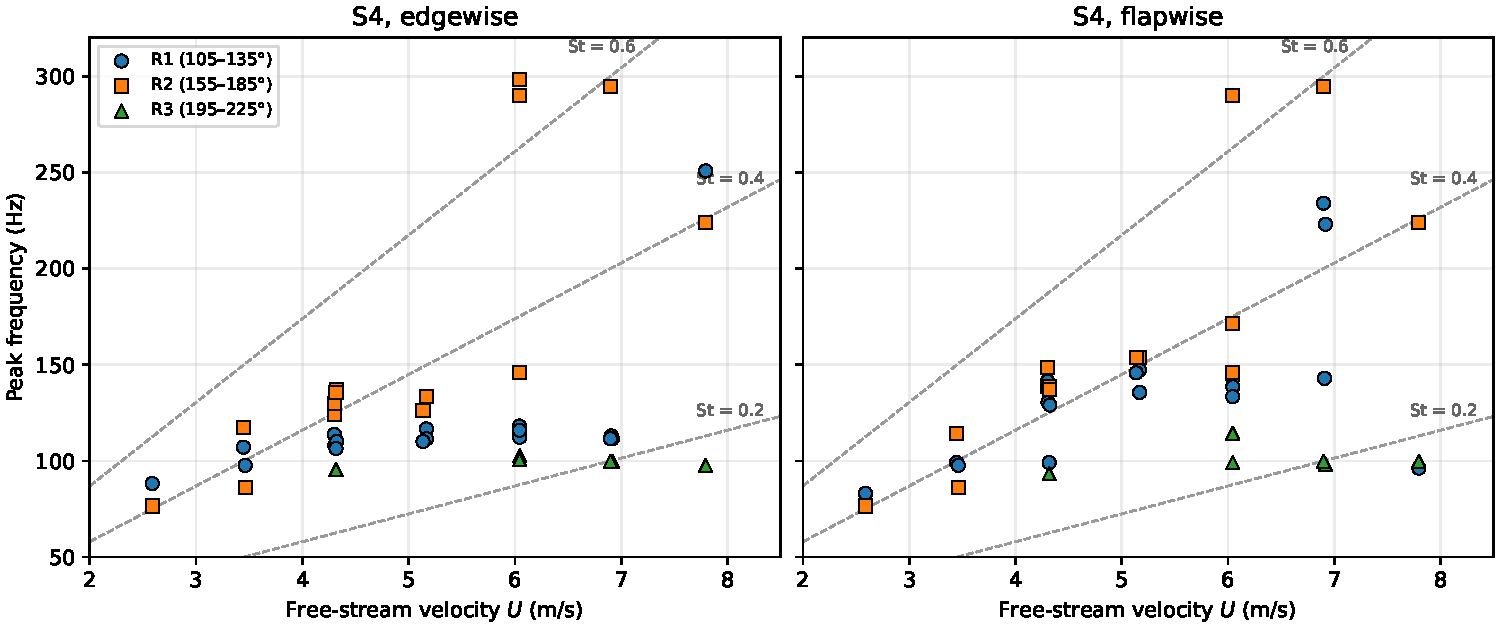
\includegraphics[width=\textwidth]{peak_vs_speed.pdf}
  \caption{Peak frequency against flow speed for every flagged run, sensor~4.
  Dashed lines: $f = St\,U/\bar{c}$ for $St = 0.2$, 0.4 and 0.6. A
  structural resonance is a horizontal row of points; a flow-driven frequency
  follows a dashed line.}
  \label{fig:speed}
\end{figure}

Figure~\ref{fig:speed} shows the main result: the regions behave
differently. R1 edgewise and R3 form horizontal rows (fixed frequency), while
most R2 points follow the $St = 0.4$ line (frequency proportional to speed).

The regions are also flagged at different flow conditions. With sensor~4, R1
and R2 are flagged from $Re = 1.0\times10^5$ upward and R3 only from
$2.2\times10^5$; sensor~1 flags all three from higher $Re$
($1.5\times10^5$ for R1 and R2, $2.9\times10^5$ for R3). Sensor~4 is at the
tip, where the blade moves most, so smaller vibrations reach the threshold
there.

\subsection{R1: fixed-frequency vibration}

\begin{figure}[H]
  \centering
  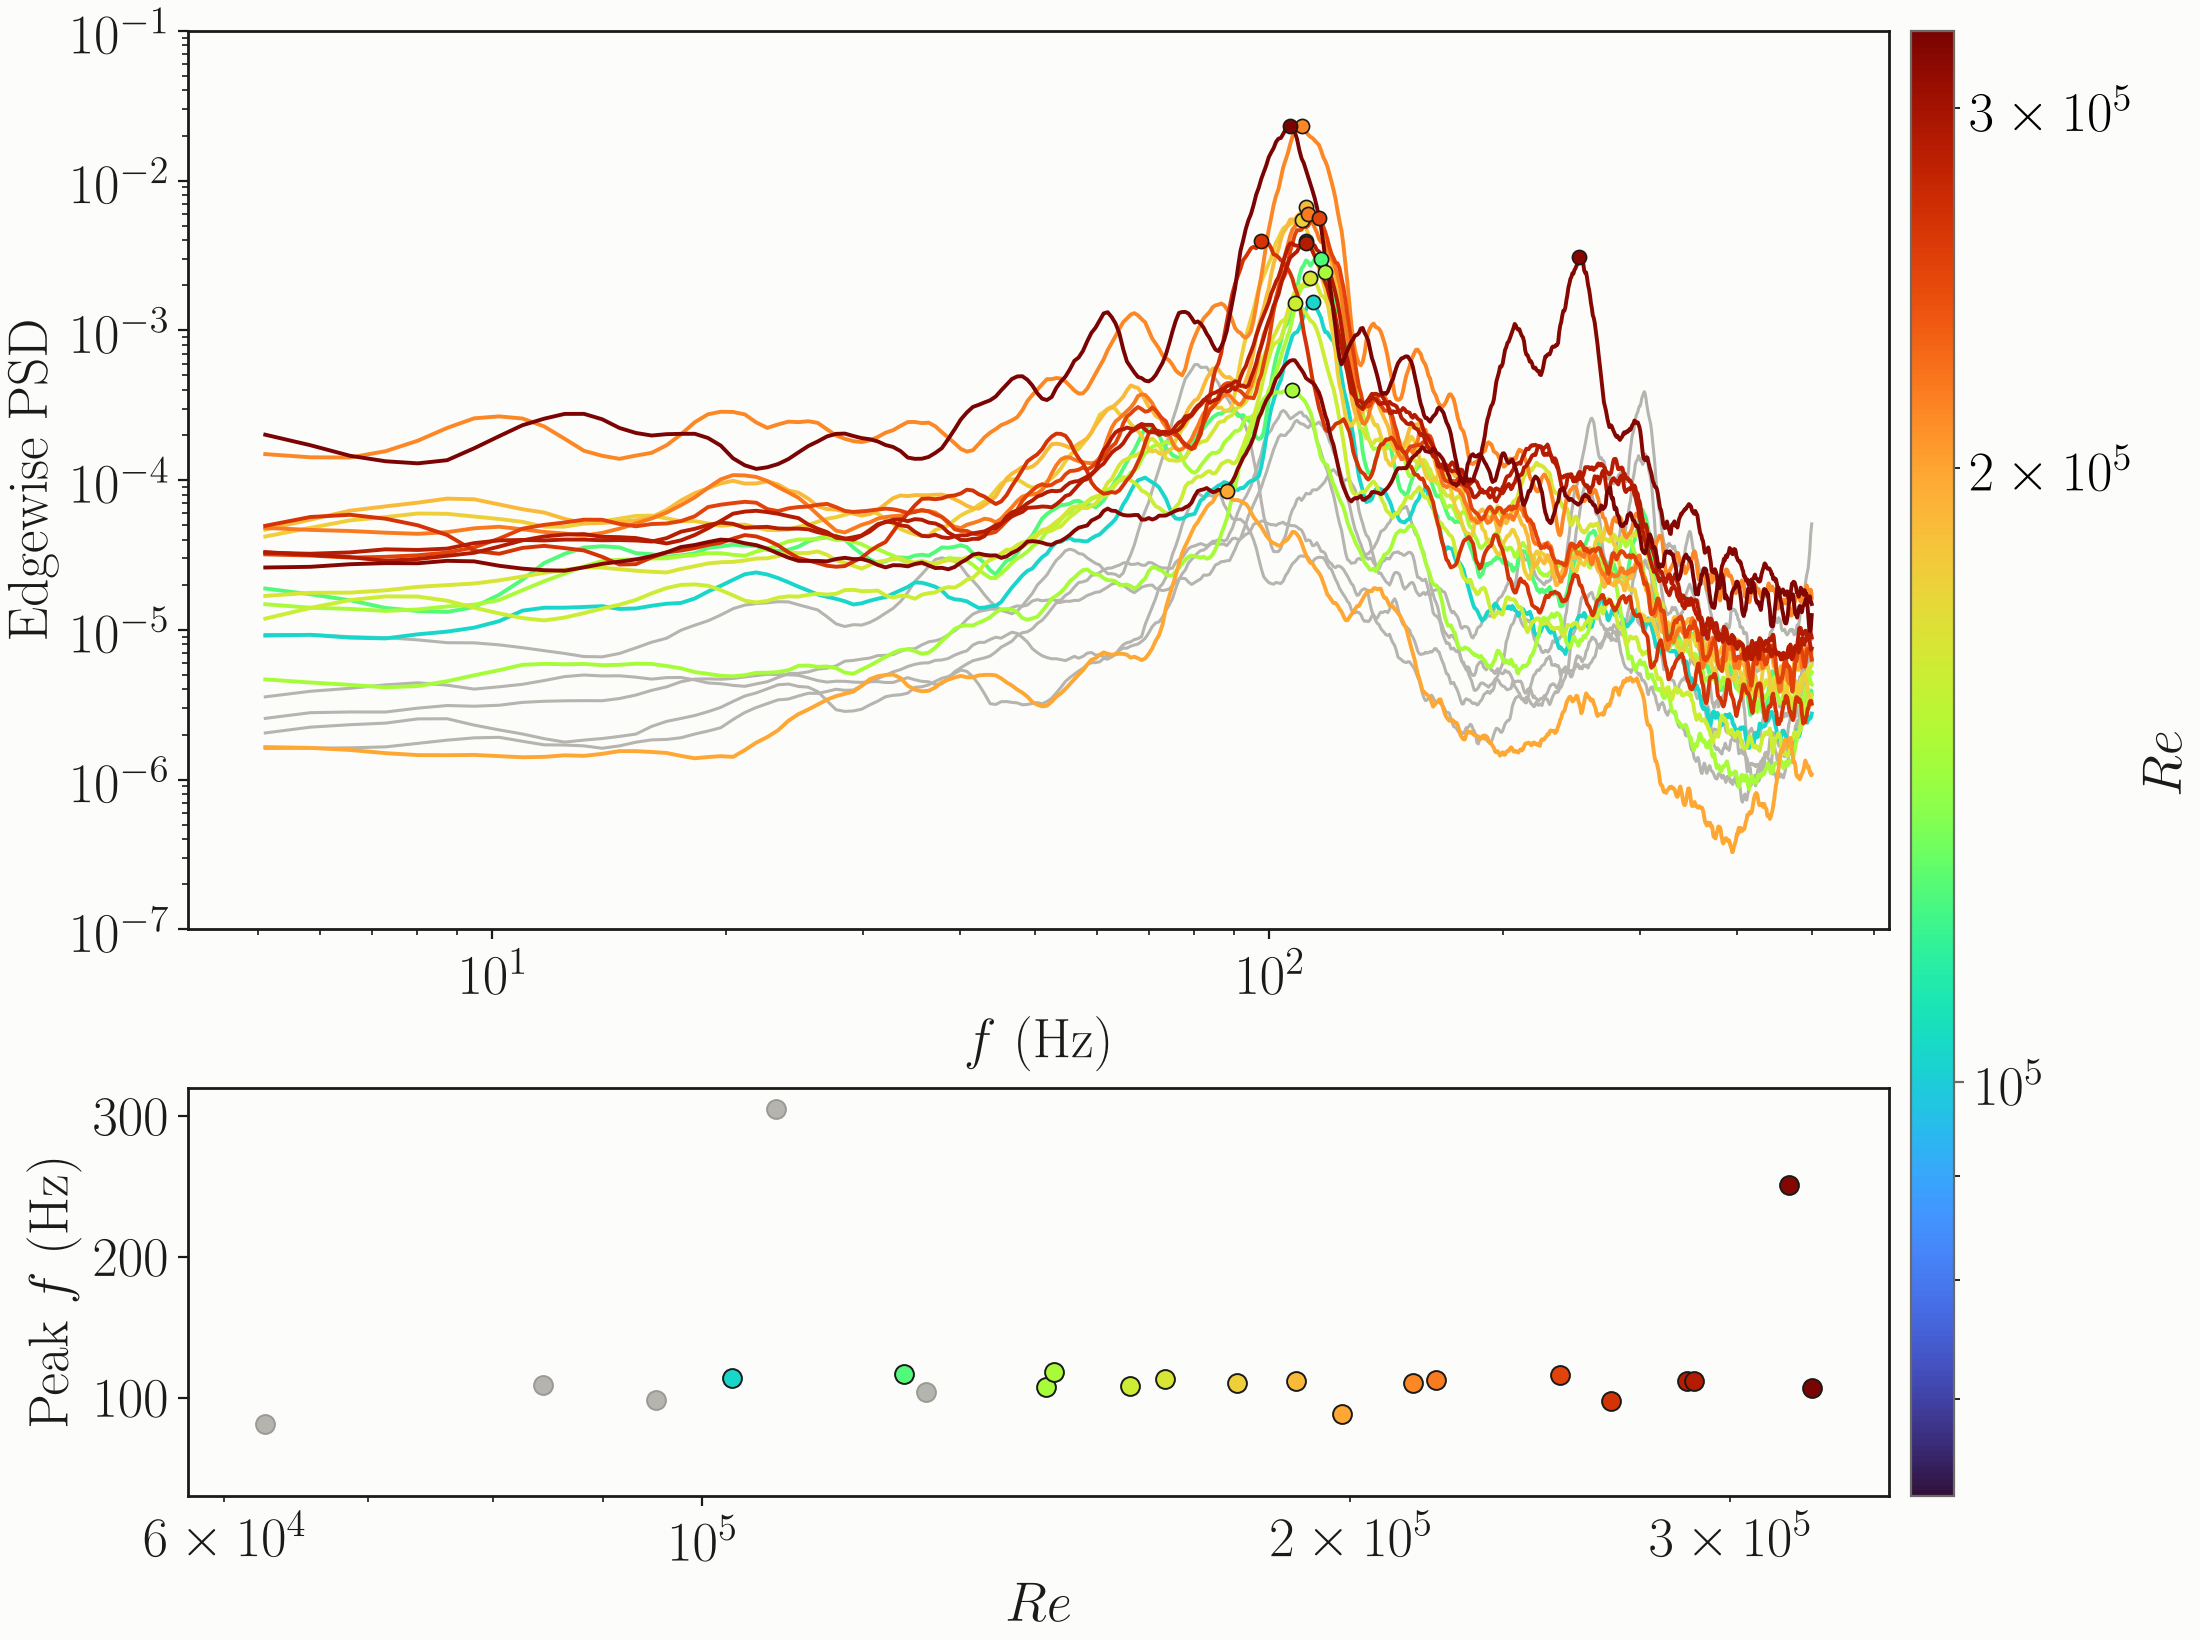
\includegraphics[width=0.49\textwidth]{S4/R1_edgewise_frequency.png}\hfill
  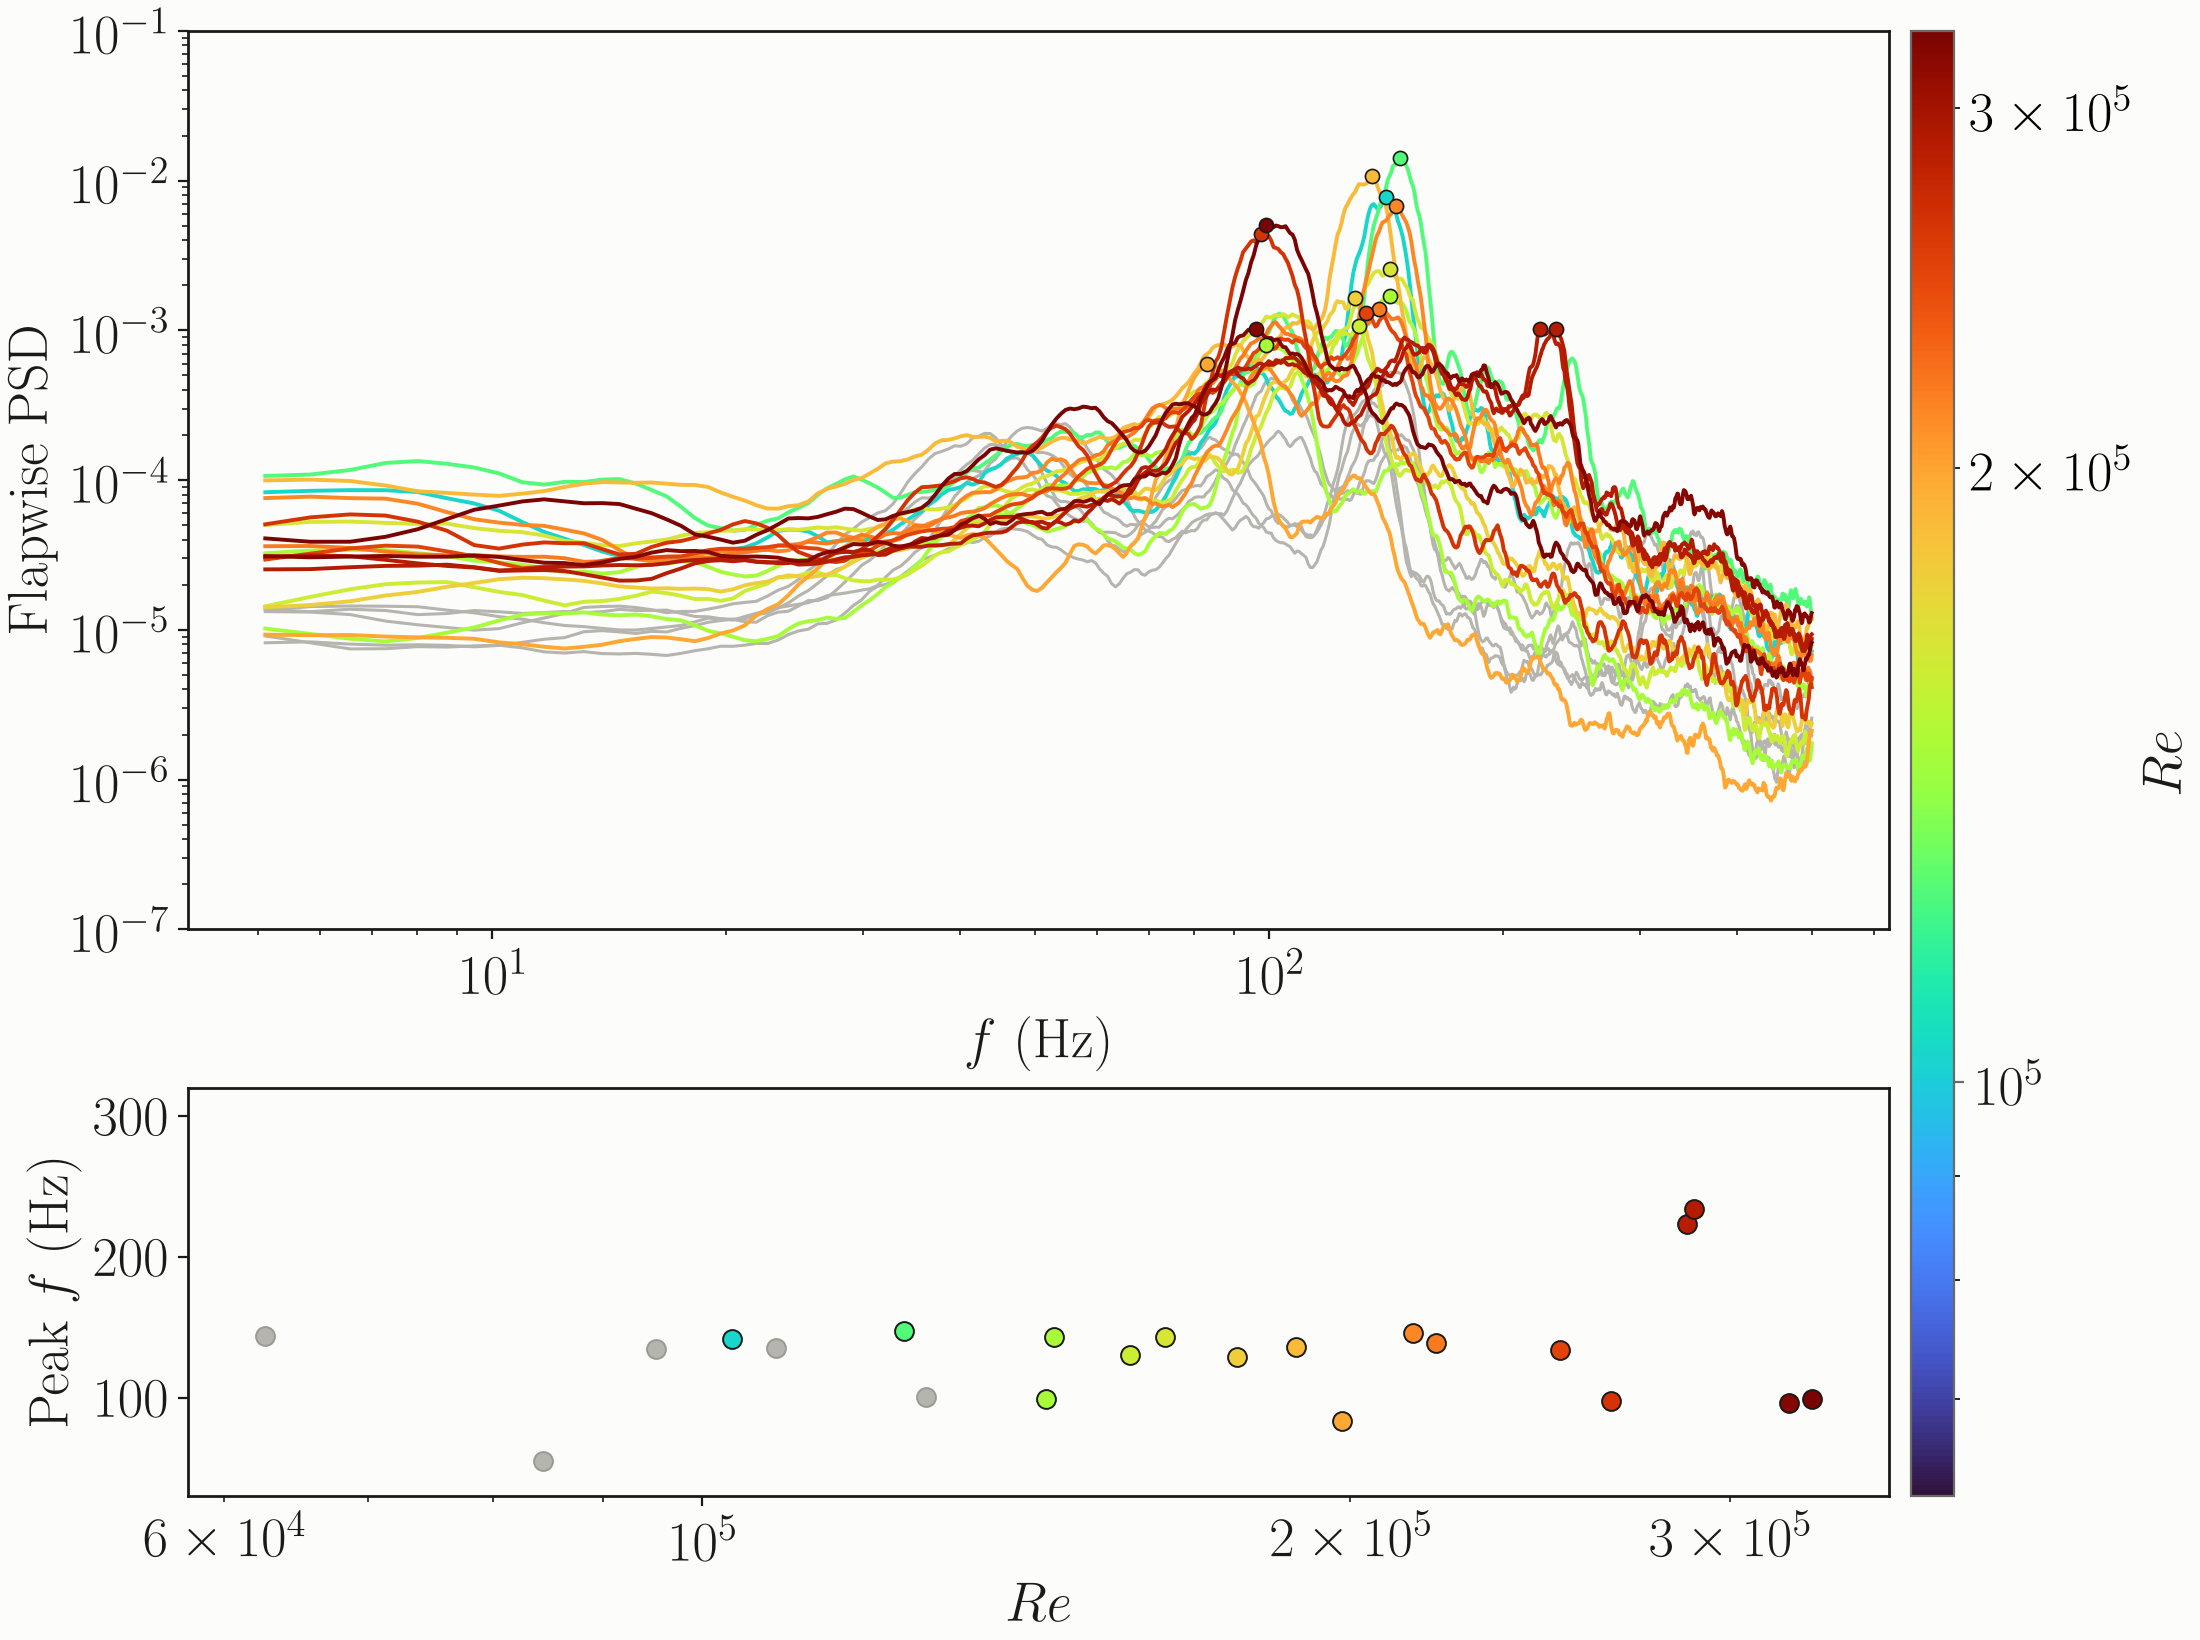
\includegraphics[width=0.49\textwidth]{S4/R1_flapwise_frequency.png}
  \caption{R1, sensor~4: edgewise (left) and flapwise (right). Top: PSD at
  each run's peak angle, coloured by $Re$ (grey: not flagged in R1). Bottom:
  peak frequency against $Re$.}
  \label{fig:r1}
\end{figure}

\paragraph{Edgewise.} The edgewise vibration in R1 has one frequency. Of the
17 flagged runs (sensor~4), the 13 below 1414\,psi all peak between 107 and
118\,Hz ($112 \pm 3$\,Hz) while $U$ goes from 3.4 to 6.9\,m/s and the
Strouhal number falls from 0.43 to 0.22. The frequency is set by the blade,
not by the flow. The three 1414\,psi runs, in the densest gas
(113\,kg/m$^3$), peak lower, at 88, 98 and 106\,Hz. The fastest run
(704\,psi, 7.8\,m/s) peaks at 251\,Hz, but the accelerometer clipped at that
angle, which distorts the spectrum, so that value is not reliable.

\paragraph{Flapwise.} The flapwise peaks fall into three groups:
\begin{itemize}
  \item 10 runs at 129--147\,Hz, across 4.3 to 6.9\,m/s and all pressures
        below 1414\,psi: again a fixed frequency, not following the flow;
  \item 5 runs at 83--99\,Hz: the three 1414\,psi runs, the slowest 704\,psi
        run (3.4\,m/s) and the fastest (7.8\,m/s, clipped);
  \item the two 704\,psi runs at 6.9\,m/s, at 223 and 234\,Hz.
\end{itemize}
The edgewise and flapwise peaks of a run are different in R1 (within 3\,Hz in
only 1 of 17 runs), so the two directions vibrate at separate frequencies,
about 112 and 140\,Hz.

\subsection{R2: flow-driven vibration}
\label{sec:r2}

\begin{figure}[H]
  \centering
  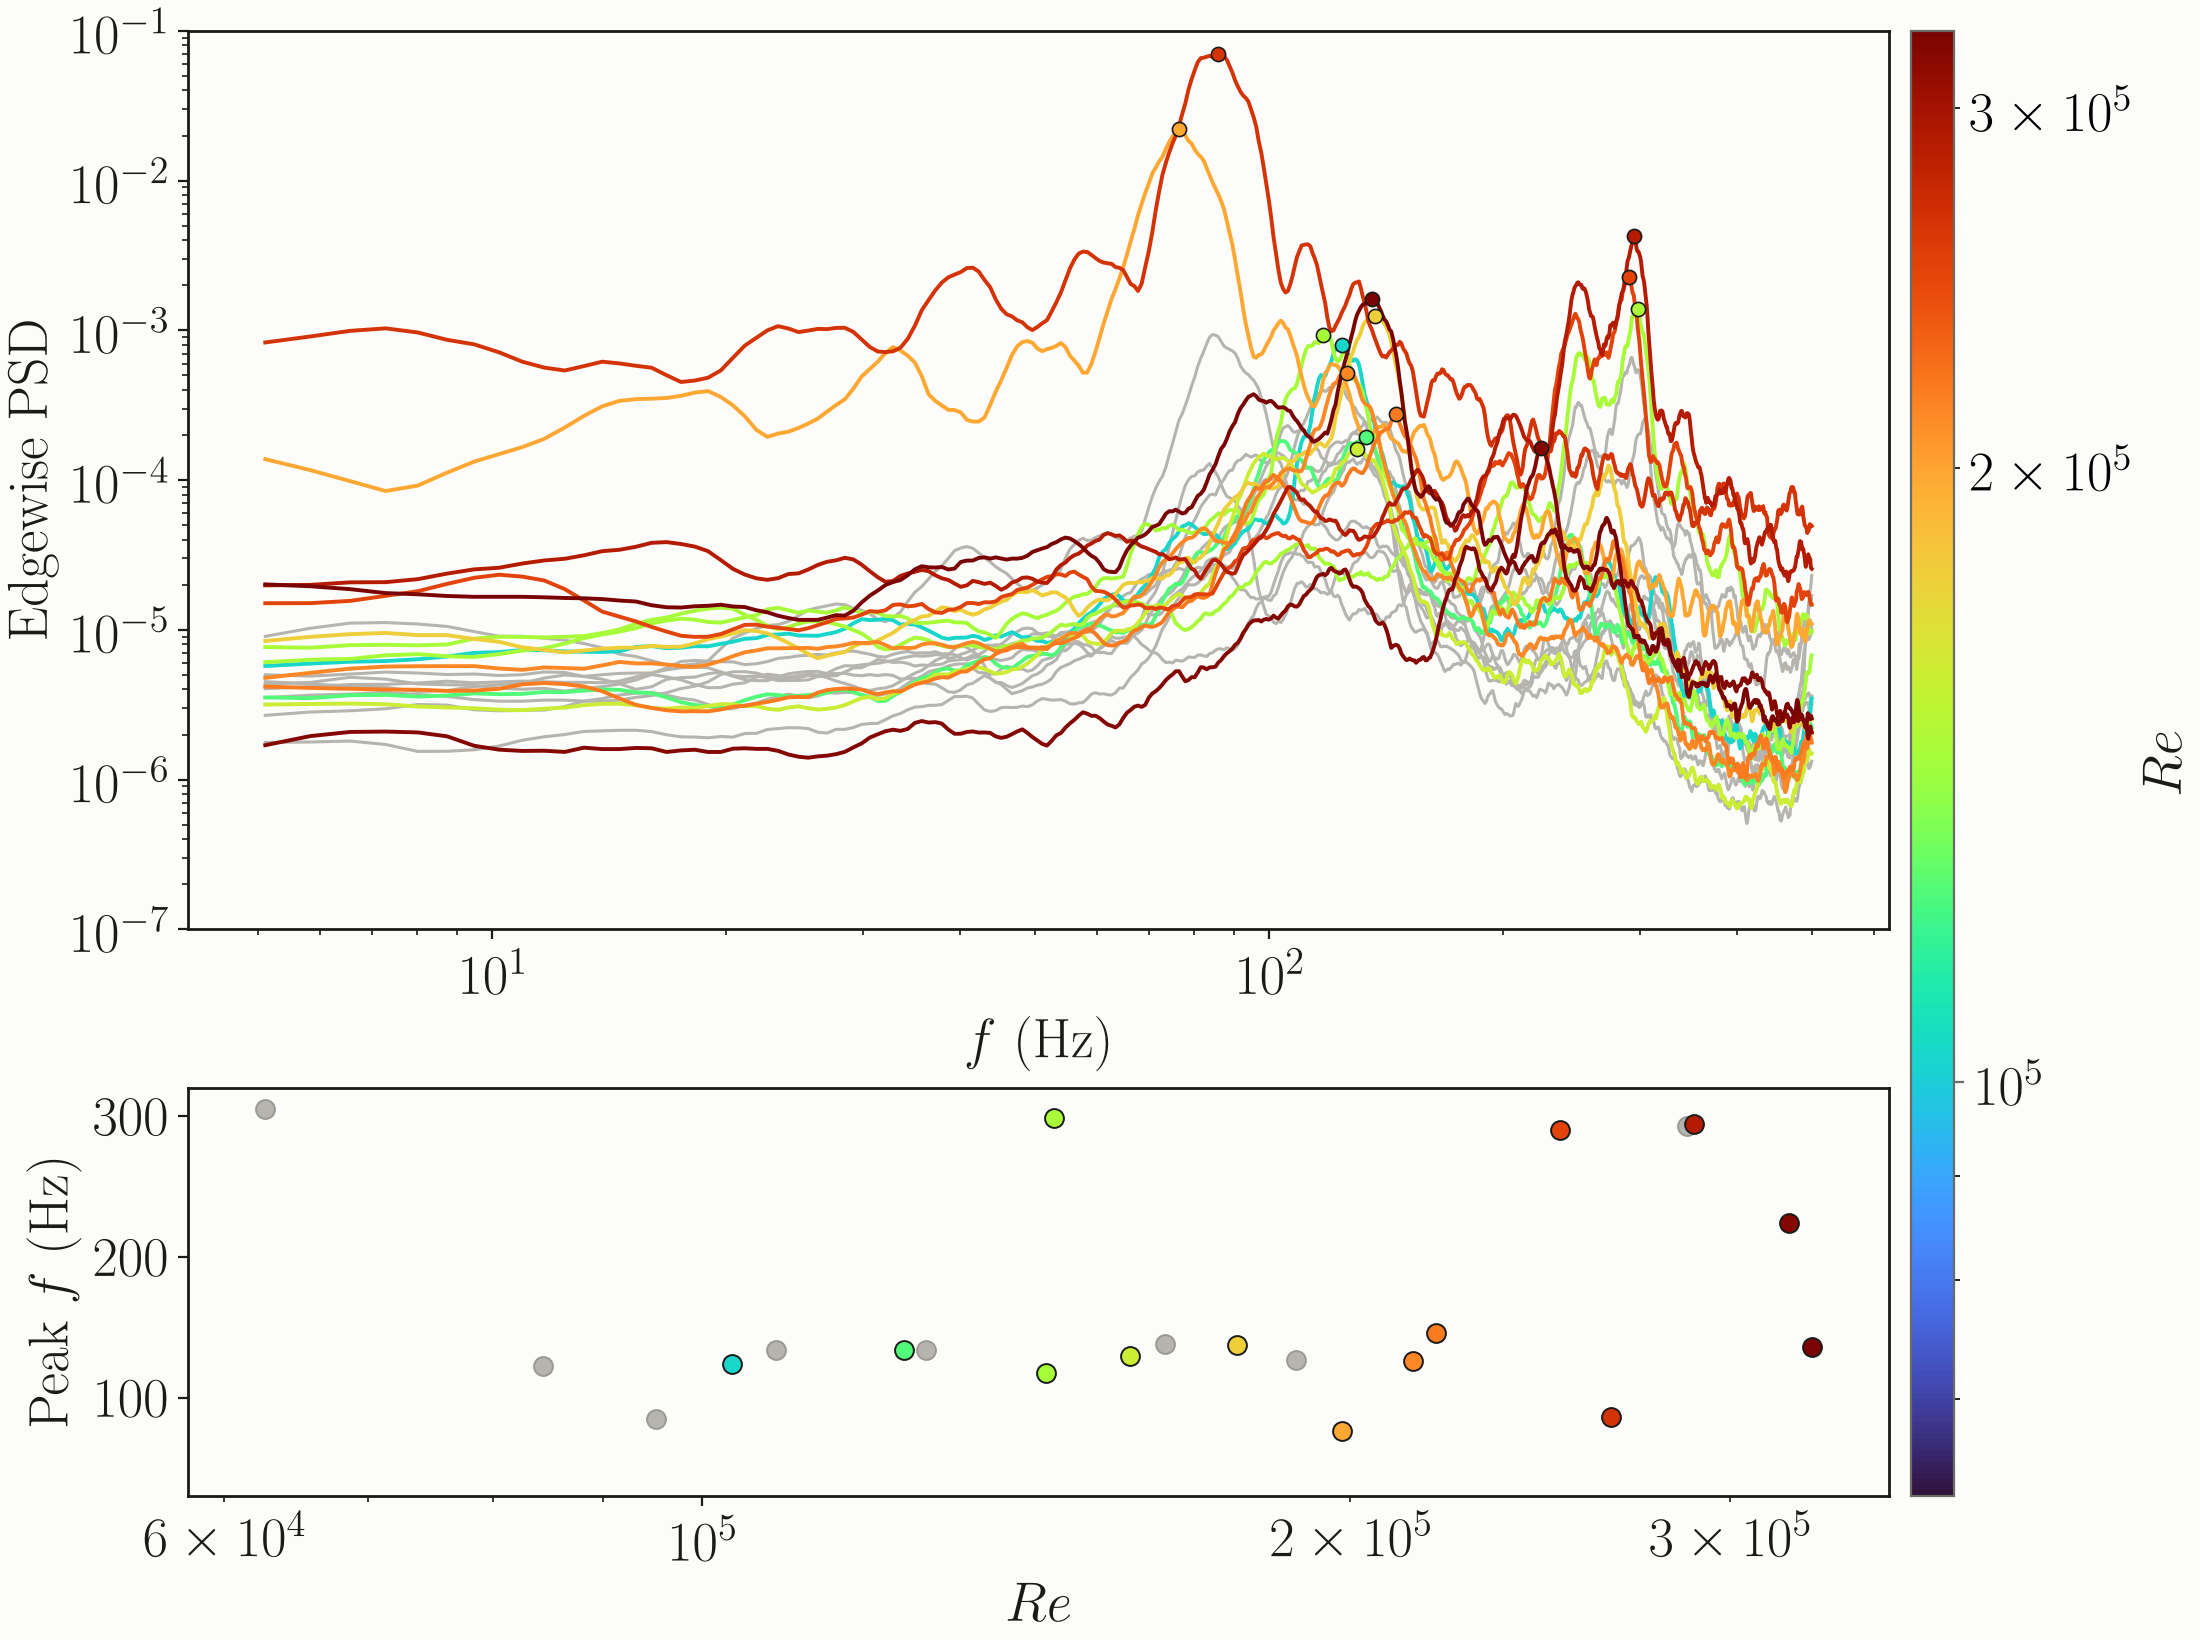
\includegraphics[width=0.49\textwidth]{S4/R2_edgewise_frequency.png}\hfill
  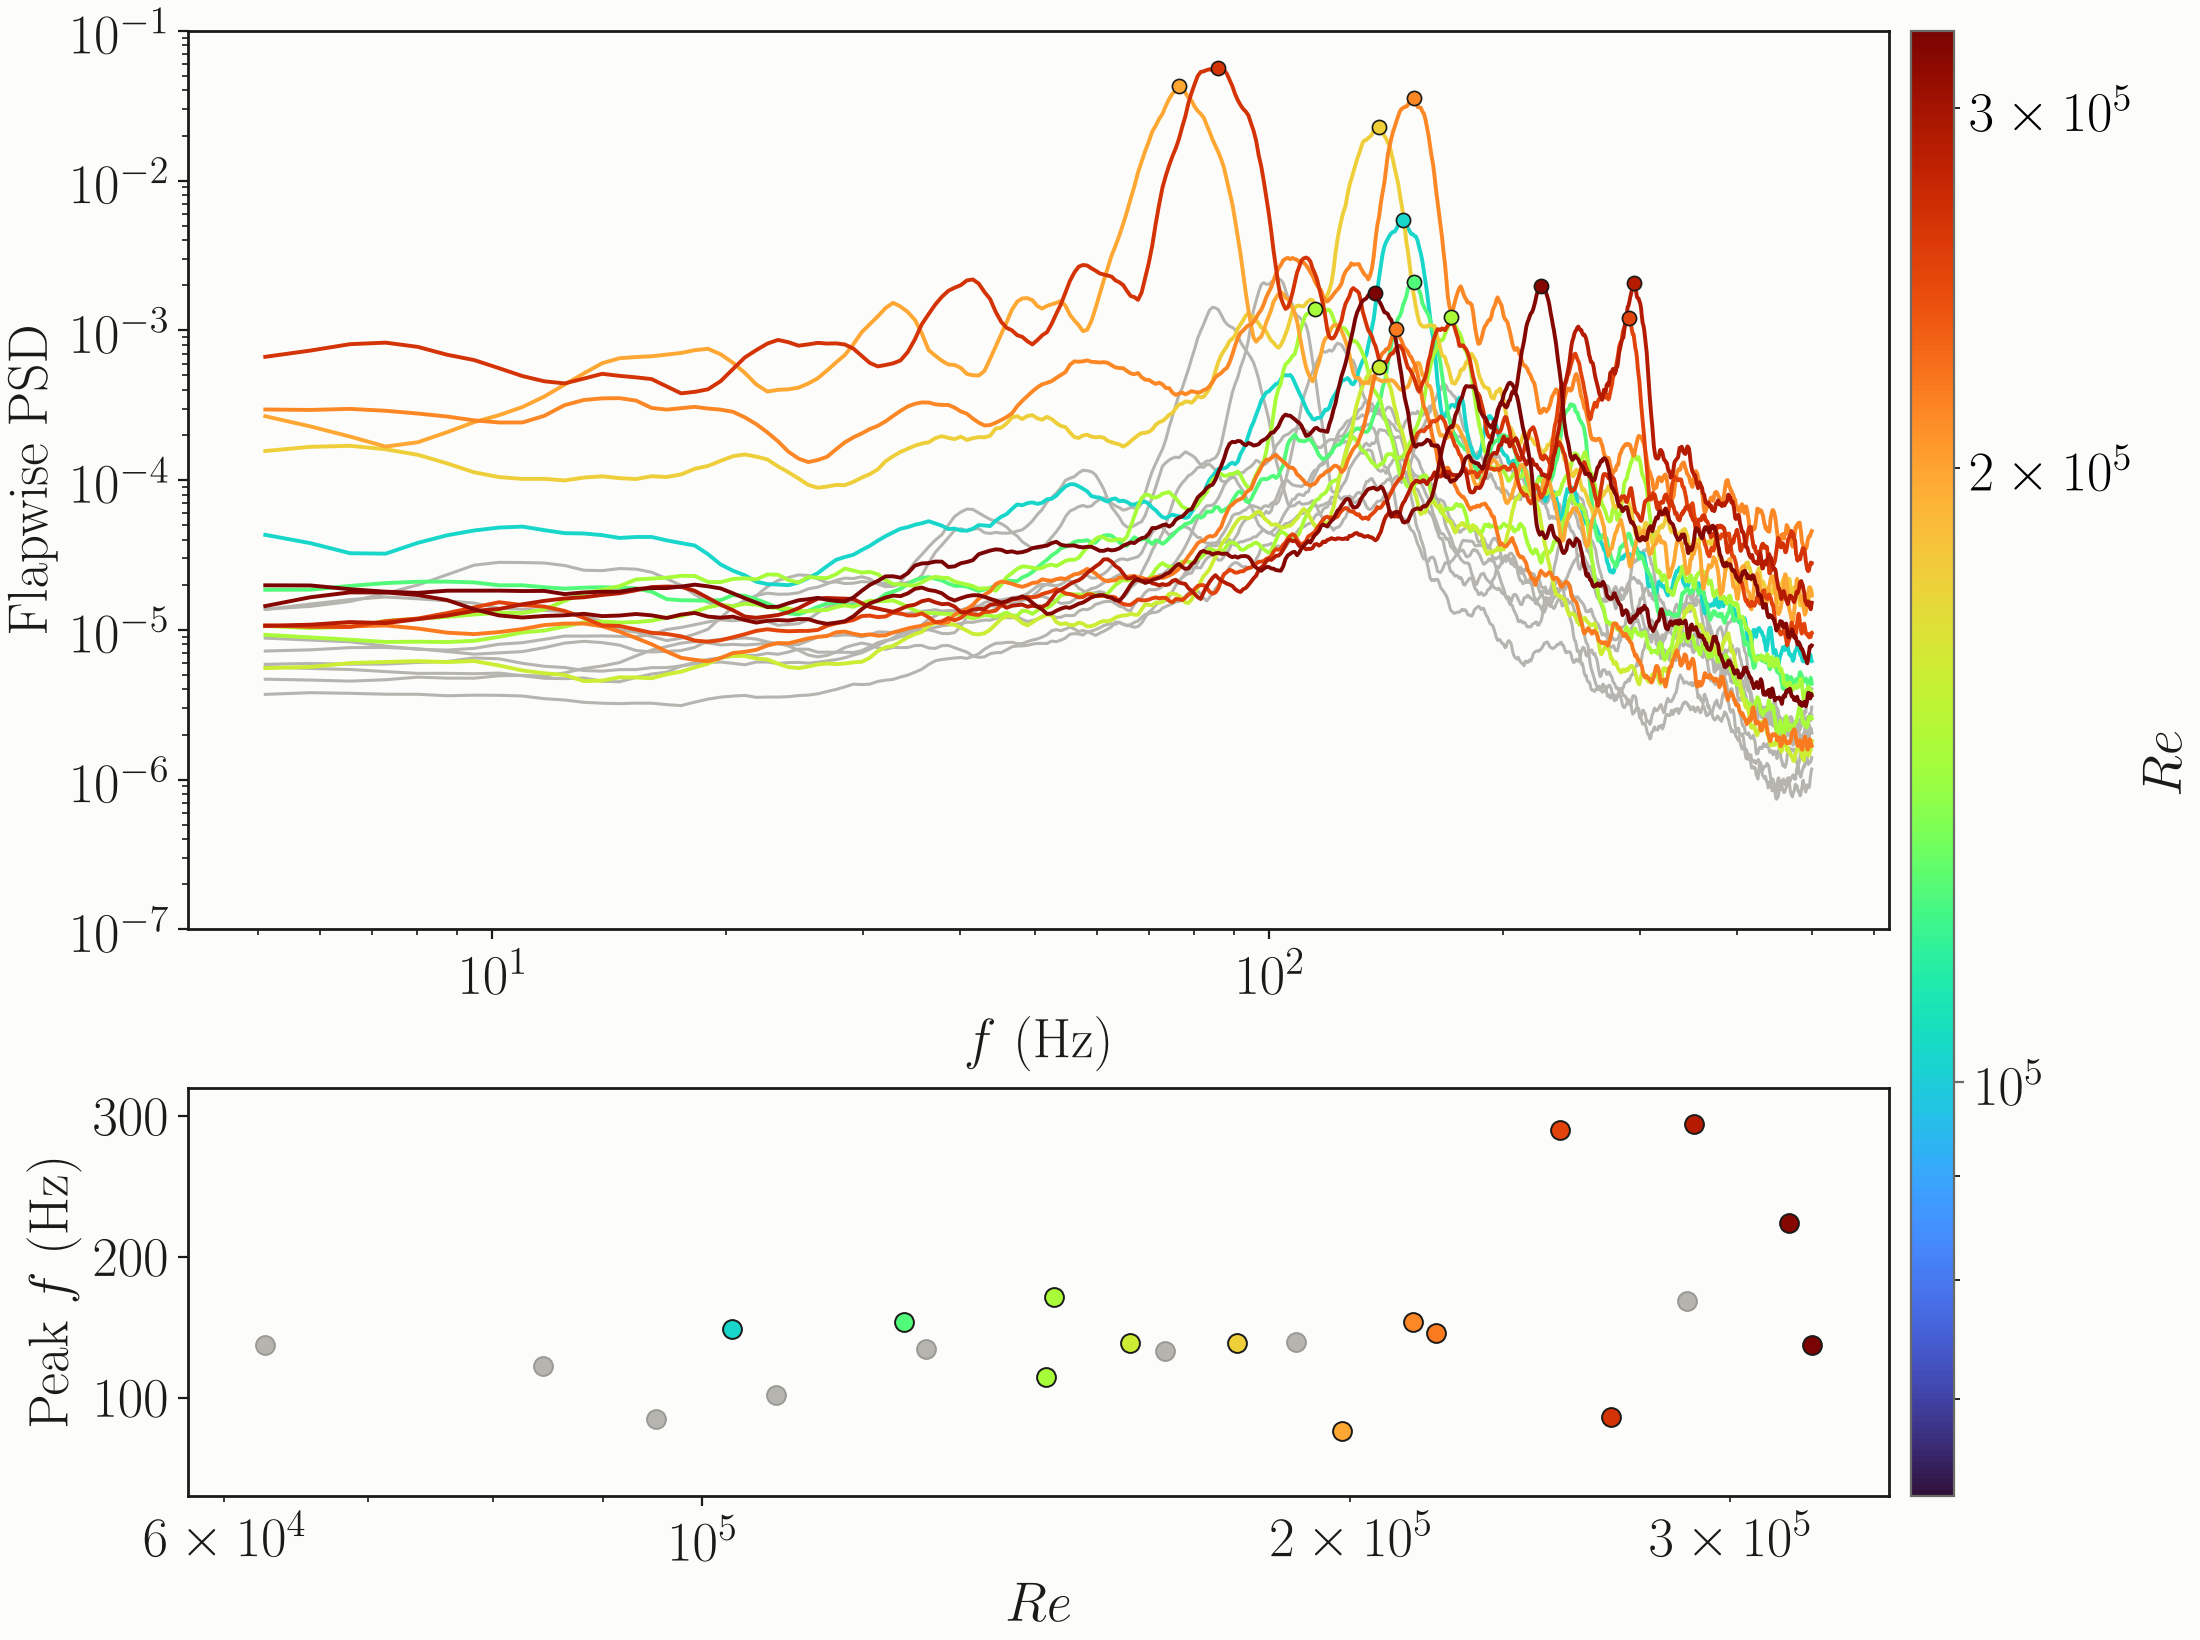
\includegraphics[width=0.49\textwidth]{S4/R2_flapwise_frequency.png}
  \caption{R2, sensor~4, in hertz: edgewise (left) and flapwise (right). The
  peak frequency rises with $Re$.}
  \label{fig:r2}
\end{figure}

\begin{figure}[H]
  \centering
  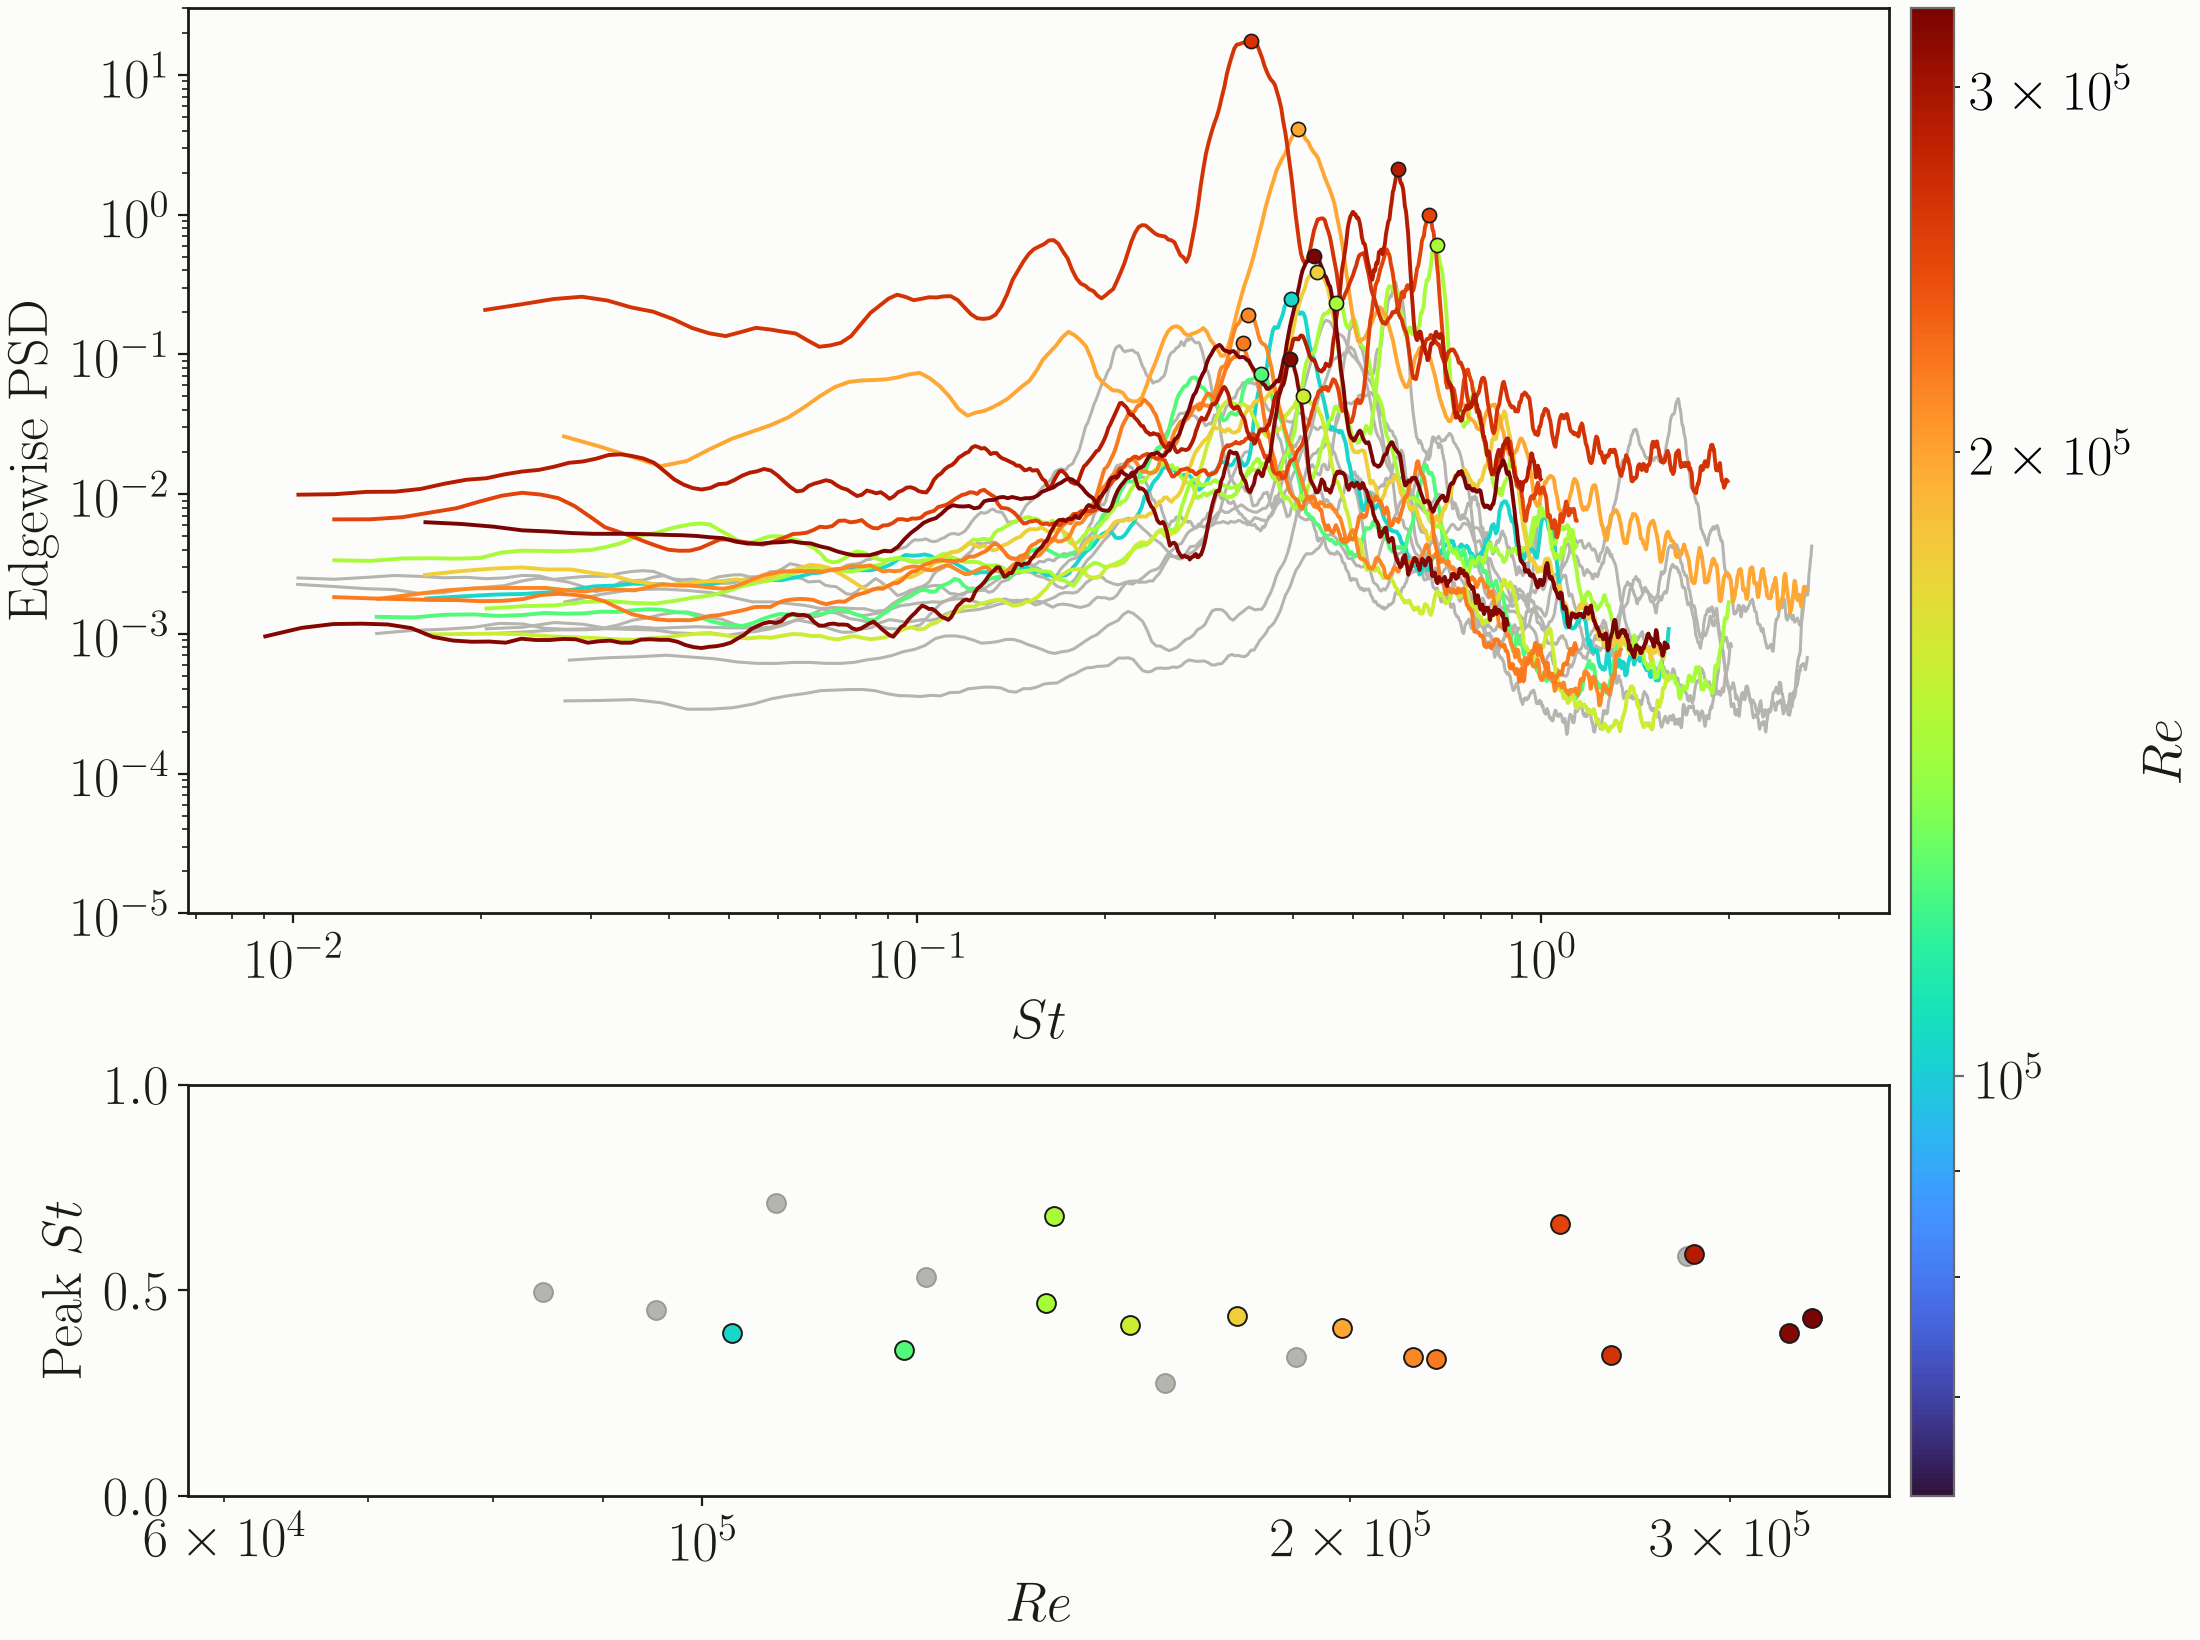
\includegraphics[width=0.49\textwidth]{S4/R2_edgewise_strouhal.png}\hfill
  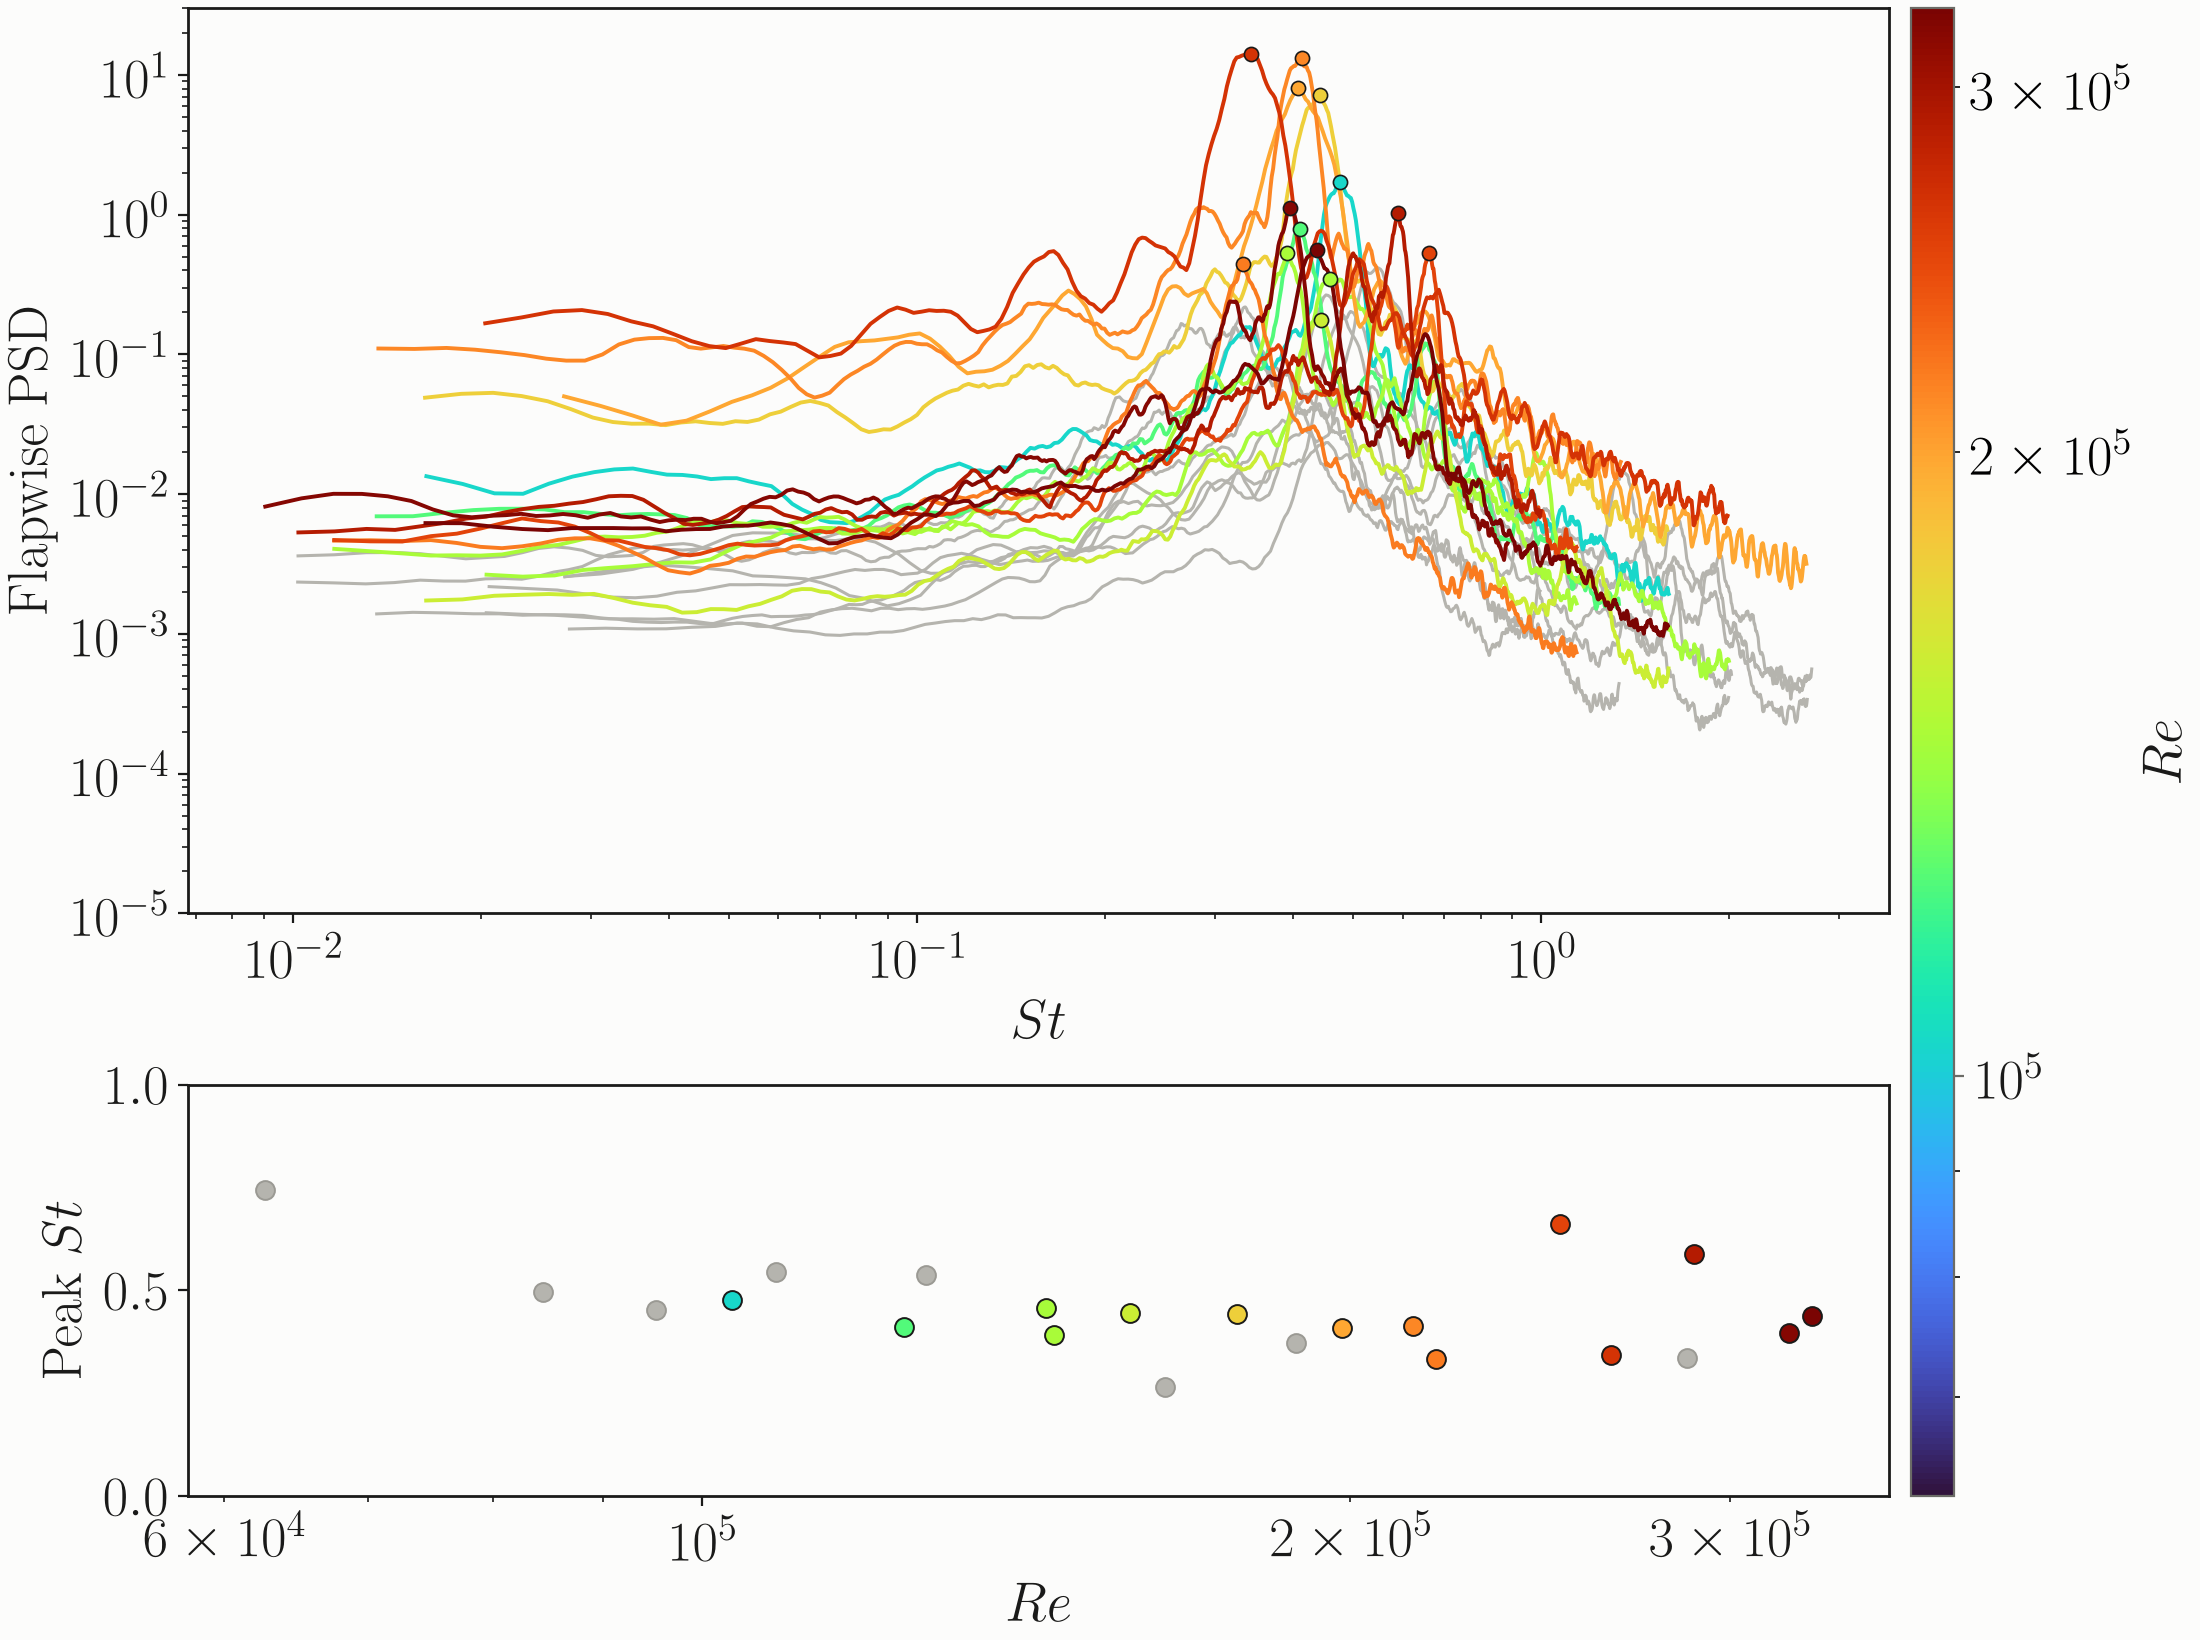
\includegraphics[width=0.49\textwidth]{S4/R2_flapwise_strouhal.png}
  \caption{R2, sensor~4, as Strouhal number: edgewise (left) and flapwise
  (right). Most peaks collapse to $St \approx 0.4$.}
  \label{fig:r2st}
\end{figure}

In R2 the peak frequency rises with flow speed (Figure~\ref{fig:r2}): from
77\,Hz at 2.6\,m/s through 86--171\,Hz at 3.4--6.0\,m/s to 224\,Hz at
7.8\,m/s. Plotted as a Strouhal number (Figure~\ref{fig:r2st}), these peaks
collapse: the 23 sensor-4 peaks below 250\,Hz have a median $St$ of 0.41 and
all lie between 0.33 and 0.48, while their frequency changes by a factor of
three. A straight-line fit gives $f = 25.2\,U + 18$\,Hz, close to the
$St = 0.4$ line ($f = 29.0\,U$). The vibration in R2 therefore follows the
flow, as expected for forcing by periodic vortex shedding, rather than
sitting at a structural frequency.

A second group does not follow this trend: three fast runs peak at
290--298\,Hz, at $St = 0.59$--0.68. The two 704\,psi runs (6.0 and
6.9\,m/s) do so in both directions, the 385\,psi run (6.0\,m/s) edgewise only;
its flapwise peak is at 171\,Hz, on the $St \approx 0.4$ trend. These peaks are not clipped. Whether they
are a higher harmonic of the shedding, a different flow feature or a
structural mode near 290\,Hz cannot be told from these runs alone.

Unlike R1, the edgewise and flapwise peaks of a run coincide in R2 (within
3\,Hz in 9 of 14 runs): the blade moves in both directions at the forcing
frequency.

The R2 medians in Table~\ref{tab:overview} differ between sensors (sensor~1:
189 and 216\,Hz; sensor~4: 135 and 147\,Hz) mainly because sensor~1 flags
fewer of the slower runs, so the $\sim$290\,Hz group makes up a larger share of
its flagged runs. For the runs both sensors flag, the R2 peaks agree to within
5\,Hz in 15 of 18 cases.

\subsection{R3: vibration at about 100 Hz in the fastest runs}

\begin{figure}[H]
  \centering
  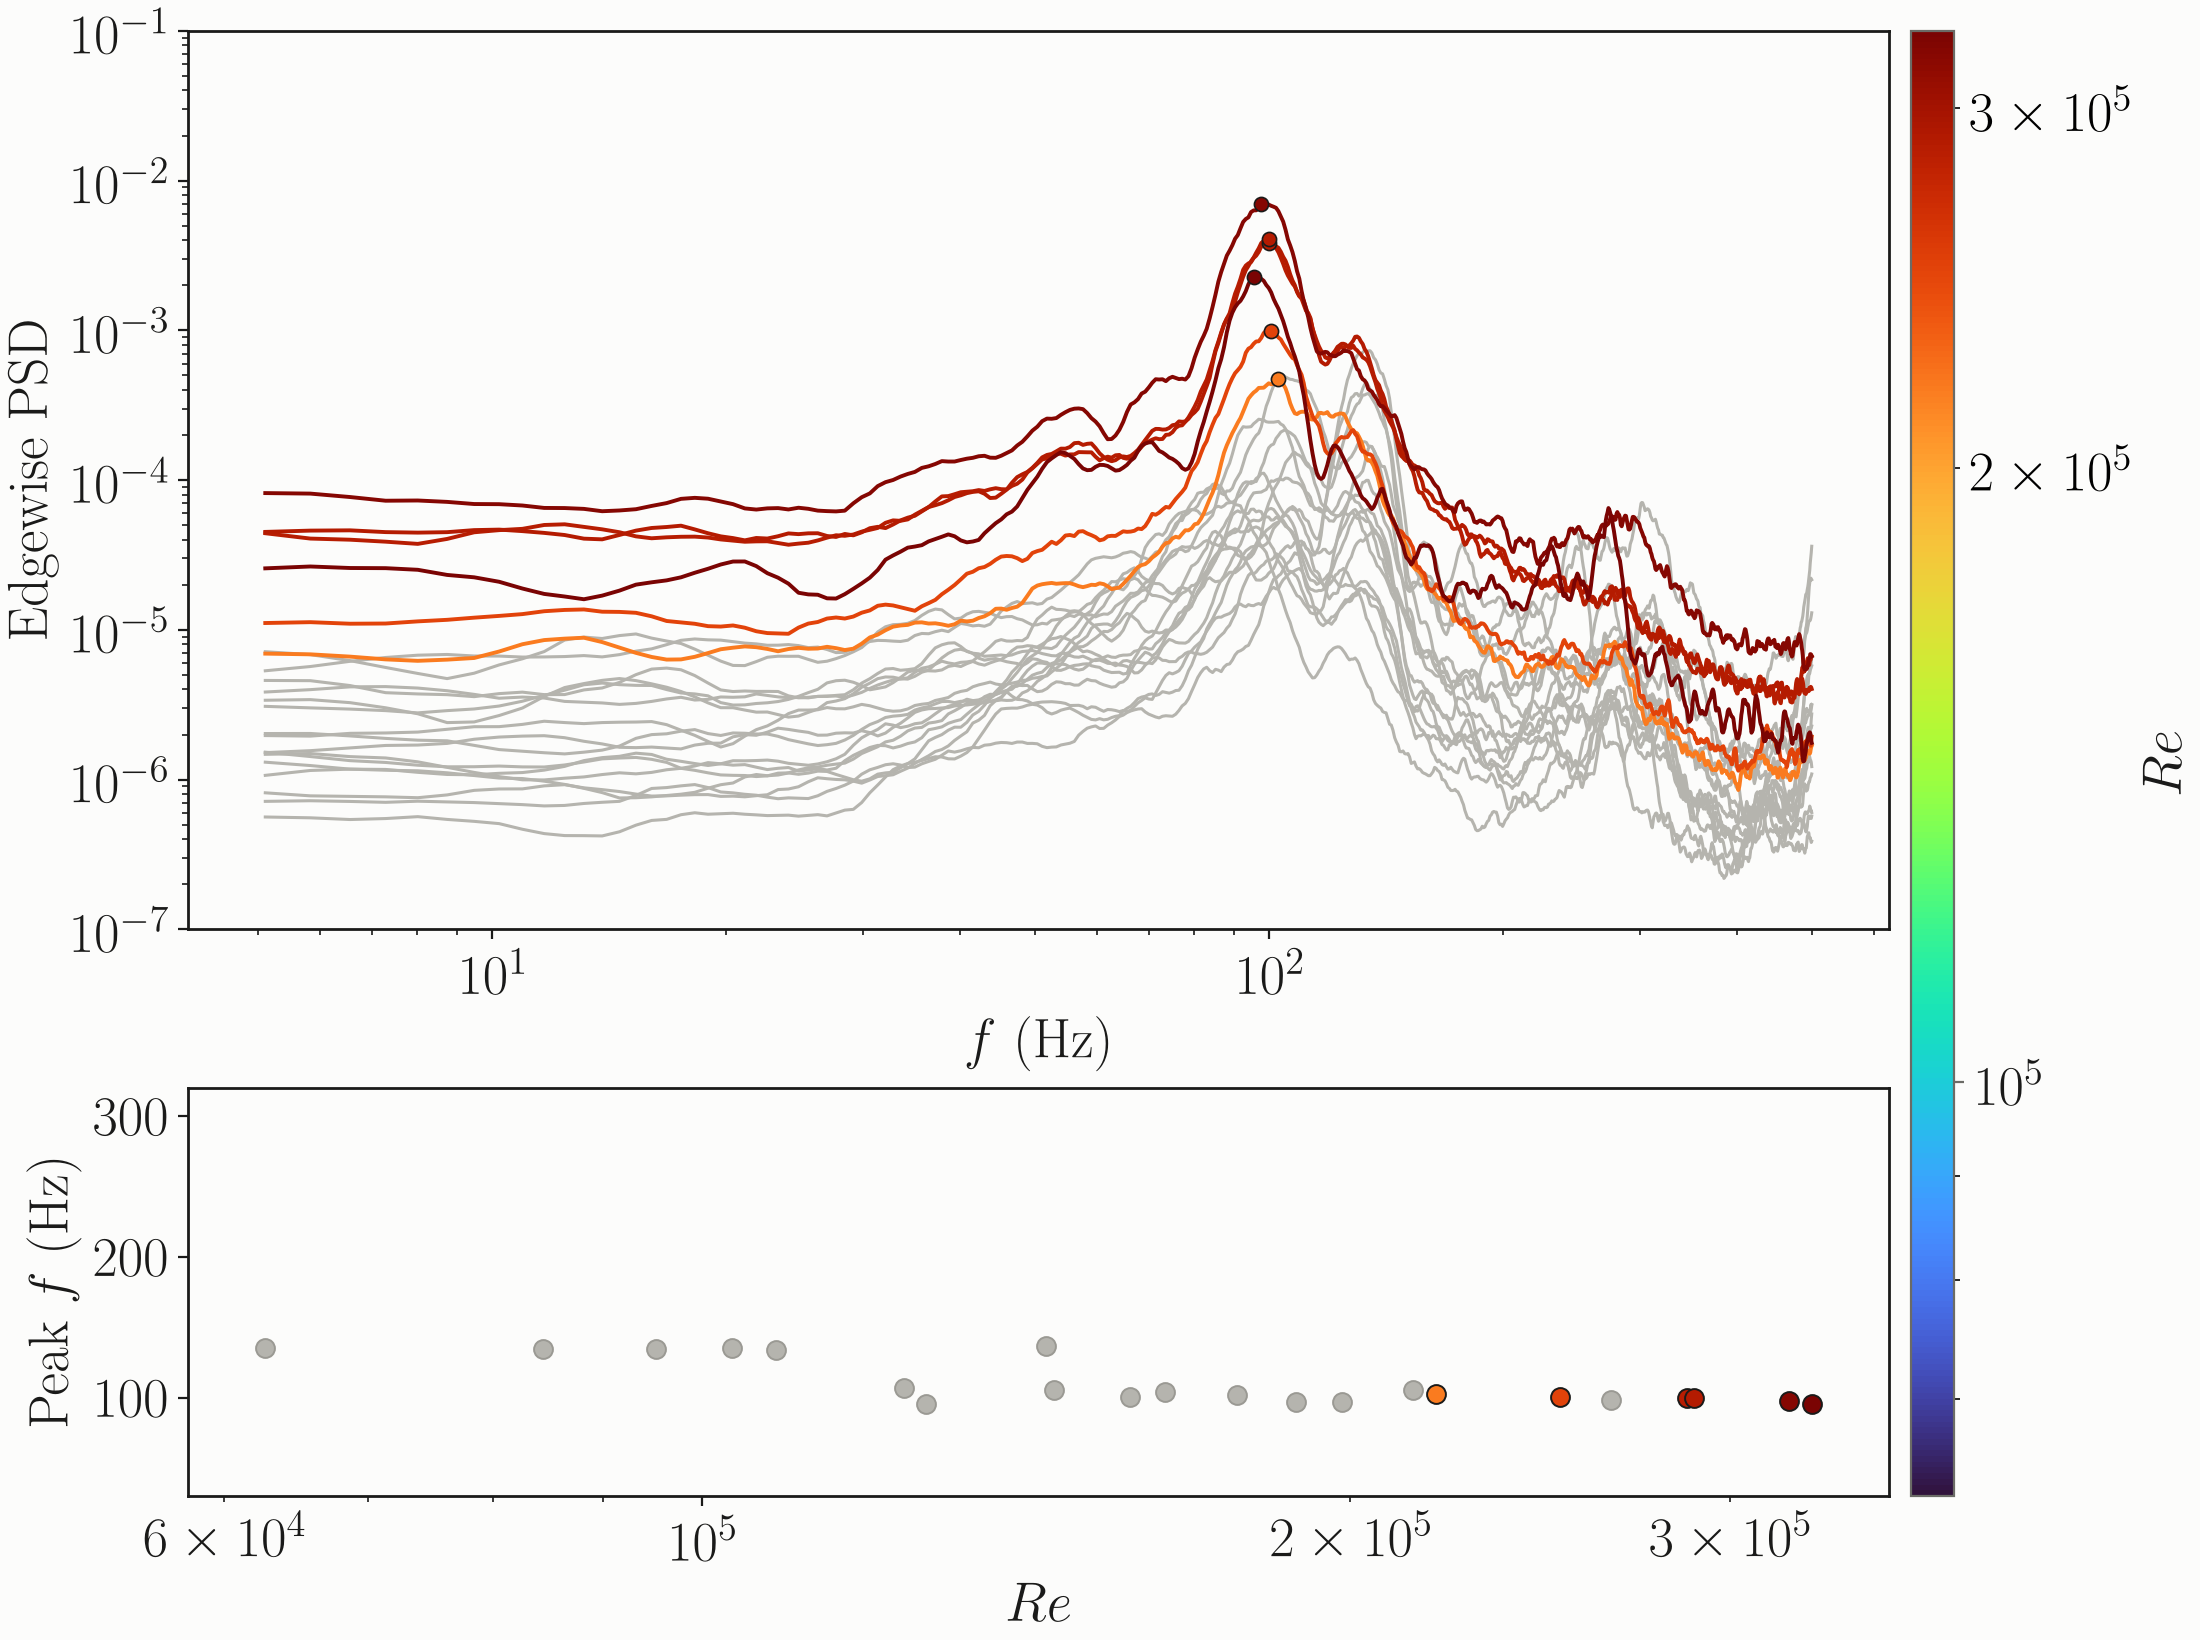
\includegraphics[width=0.49\textwidth]{S4/R3_edgewise_frequency.png}\hfill
  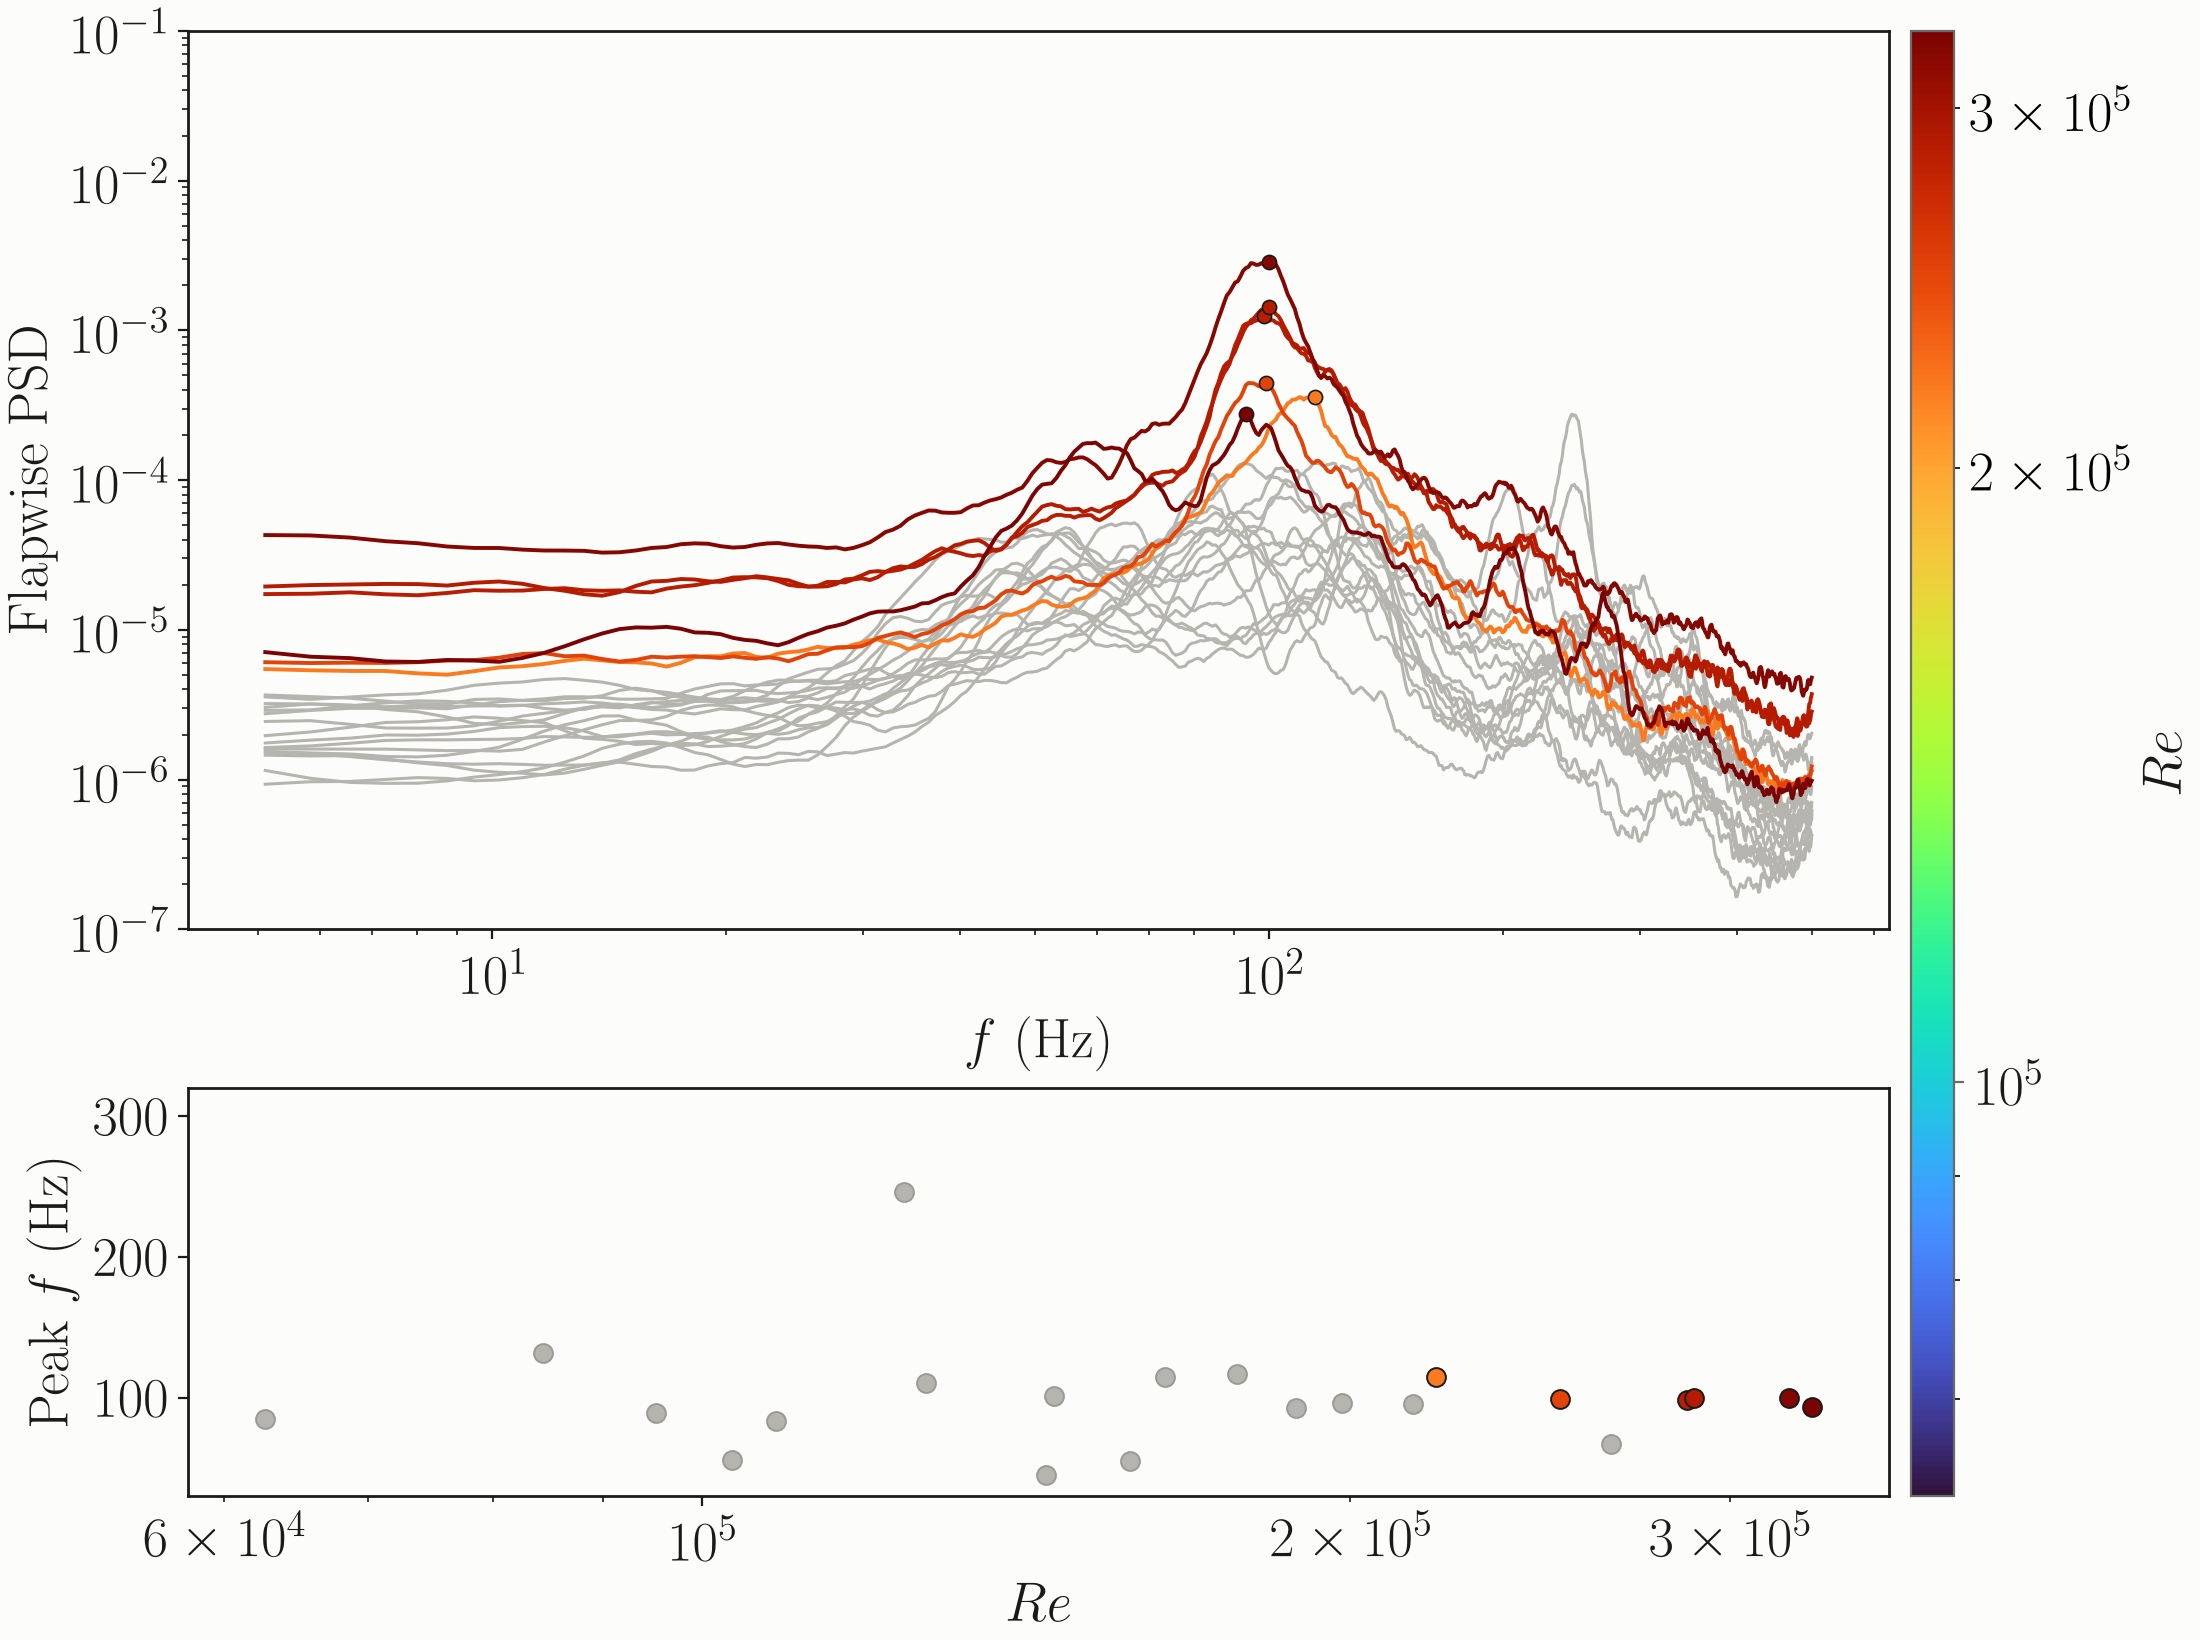
\includegraphics[width=0.49\textwidth]{S4/R3_flapwise_frequency.png}
  \caption{R3, sensor~4: edgewise (left) and flapwise (right).}
  \label{fig:r3}
\end{figure}

R3 is flagged in only six runs with sensor~4 (four with sensor~1), all fast or
dense: 605\,psi at 6.0\,m/s, 704\,psi at 6.0--7.8\,m/s and 1414\,psi at
4.3\,m/s. All peak at $100 \pm 5$\,Hz (93--114\,Hz) in both directions, while
$U$ ranges from 4.3 to 7.8\,m/s and $St$ falls from 0.31 to 0.17. Like R1,
this is a fixed frequency set by the structure. The edgewise and flapwise
peaks coincide (within 3\,Hz in 5 of 6 runs), so the blade moves in both
directions at the same frequency. Four of the twelve R3 peaks (three runs, all
704\,psi at 6.9--7.8\,m/s) come from angles where sensor~4 clipped; their
frequencies match the unclipped ones.

\subsection{Sensor 1 compared with sensor 4}

Sensor~4 flags more runs than sensor~1 (17, 14 and 6 against 11, 10 and 4 in
R1, R2 and R3), the extra ones all at lower $Re$, because the tip moves more
than the root. For the 48 (region, direction, run) cases flagged by both, the
two sensors find the same peak to within 5\,Hz in 37:
\begin{itemize}
  \item R1 edgewise 10 of 11, R2 15 of 18 and R3 7 of 8 agree, and the median
        frequencies in R1 and R3 agree to within 2\,Hz
        (Table~\ref{tab:overview}).
  \item R1 flapwise agrees in only 5 of 11. In three runs (385\,psi at
        6.0\,m/s, 704\,psi at 4.3\,m/s, 605\,psi at 6.0\,m/s) the root sensor
        peaks at 102--109\,Hz, near the edgewise frequency, while the tip
        sensor peaks at 129--143\,Hz. Near the root the flapwise axis is
        dominated by the edgewise vibration, which is why the tip sensor is
        the better measure of the flapwise frequency.
\end{itemize}
The S1 and S4 figure sets (\code{figures/psd\_analysis} and
\code{figures/psd\_analysis/S4}) otherwise show the same patterns. The $Ca_e$-coloured sets (\code{cauchy/}) show the same peaks
coloured by the Cauchy number instead of $Re$; because $Re$ and $Ca_e$ rise
together in this test matrix, the colouring does not separate them.

\subsection{Limitations}

\begin{itemize}
  \item \textbf{One angle per run.} Each run contributes the spectrum at its
        strongest-vibrating angle in the window, so a run whose vibration
        changes character across the window is represented by one point.
  \item \textbf{Clipping.} Twelve of the 74 flagged sensor-4 peaks come from
        angles where the accelerometer reached its $\pm16\,g$ limit. Their
        frequencies agree with unclipped runs except for the 251\,Hz R1
        edgewise peak of the fastest run.
  \item \textbf{High frequencies.} Peaks above $\sim$150\,Hz (the R1 flapwise
        $\sim$230\,Hz and R2 $\sim$290\,Hz groups) are uncertain by up to
        15\,Hz because of the sample-rate uncertainty.
  \item \textbf{$Re$ and $Ca_e$ are not independent.} Both rise with speed
        and pressure, so these data cannot separate a Reynolds-number effect
        from a load effect.
  \item \textbf{Natural frequencies.} Until the mount configuration of the
        production runs is settled, the fixed frequencies of R1
        ($\sim$112 and $\sim$140\,Hz) and R3 ($\sim$100\,Hz) cannot be
        assigned to specific modes of the blade.
\end{itemize}

\paragraph{Reproducing.} The PSD figures are made by \code{plot\_psd.py}
(\code{--mode runs}, sensors S1 and S4, \code{--region 120 170 210},
\code{--component y z}, \code{--xaxis freq st}, the 22 full-sweep runs).
\code{python3 reports/psd\_analysis/make\_figures.py} from the repository root
makes Figure~\ref{fig:speed} and prints every number quoted here from the
per-run tables next to the PSD figures.

\end{document}
